\documentclass[utf8, zavrsni]{fer}
\usepackage{booktabs}

% \usepackage{natbib}


% ==== za algo pseudokod
\usepackage{amsmath}
%\usepackage[chapter]{algorithm}
% \usepackage{algorithmic}
\usepackage{tikz,float}
\usepackage{minted}
\usemintedstyle{borland}
\usepackage{menukeys}
\usepackage{dirtytalk}

\usepackage{hyperref}
% \hypersetup{
%     colorlinks,
%     citecolor=black,
%     filecolor=black,
%     linkcolor=black,
%     urlcolor=black
% }
\hypersetup{
    bookmarks=true,         % show bookmarks bar?
    unicode=false,          % non-Latin characters in Acrobat’s bookmarks
    pdftoolbar=true,        % show Acrobat’s toolbar?
    pdfmenubar=true,        % show Acrobat’s menu?
    pdffitwindow=false,     % window fit to page when opened
    pdfstartview={FitH},    % fits the width of the page to the window
    pdftitle={My title},    % title
    pdfauthor={Author},     % author
    pdfsubject={Subject},   % subject of the document
    pdfcreator={Creator},   % creator of the document
    pdfproducer={Producer}, % producer of the document
    pdfkeywords={keyword1, key2, key3}, % list of keywords
    pdfnewwindow=true,      % links in new PDF window
    colorlinks=false,       % false: boxed links; true: colored links
    linkcolor=red,          % color of internal links (change box color with linkbordercolor)
    citecolor=green,        % color of links to bibliography
    filecolor=magenta,      % color of file links
    urlcolor=cyan,           % color of external links
    urlbordercolor={1 1 1}  % color of border around links
}

\graphicspath{{img/}}

\begin{document}

% TODO: Navedite broj rada.
\thesisnumber{000}

% TODO: Navedite naslov rada.
\title{Lanac stranica i distribuirano suglasje u sustavima elektroničkog novca}

% TODO: Navedite vaše ime i prezime.
\author{Bernard Crnković}

\maketitle

% Ispis stranice s napomenom o umetanju izvornika rada. Uklonite naredbu \izvornik ako želite izbaciti tu stranicu.
% \izvornik

% Dodavanje zahvale ili prazne stranice. Ako ne želite dodati zahvalu, naredbu ostavite radi prazne stranice.
\zahvala{}

\tableofcontents

% =========================
\chapter{Uvod}
Uslijed procesa globalizacije javlja se sve veća potreba za univerzalnim protokolom novca koji bi zamijenio ili barem objedinio postojeće lokalne bankarske sustave. Zbog loše standardizacije te njene slabe primjene u praksi, javljaju se brojni problemi u poslovanjima banaka što značajno smanjuje propusnost obrade transakcija. Također, mikrotransakcije osjetno su neisplative u sustavima koji imaju visoke naknade za prijenos. Te naknade idejno odgovaraju količini posla za uslugu koju nudi birokratski aparat banke. Cilj je minimizirati i automatizirati količinu posla koji se mora obaviti kako bi mogli vršiti razmjenu novca. Motivirani problemima aktualnih sustava, razmotrit ćemo ideju rješenja trenutnog problema --- lanac stranica.

\section{Koncept središnjeg autoriteta}
Pojam \textbf{središnjeg autoriteta} opisuje agenciju ili organizaciju koja osigurava provođenje zakona na međunarodnoj razini\cite{enwiki:969028445}. U ovom nas kontekstu konkretno zanima što taj pojam znači u računarstvu. To je najbolje demonstrirati primjerom koji je u ovoj domeni najčešće asociran s ulogom središnjeg autoriteta: \textbf{Certifikatni autoritet} (engl. \textit{Certificate authority}) - aktor koji se bavi potpisivanjem SSL certifikata korištenih u HTTPS protokolu. On ima korijenski samo-potpisani certifikat koji koristi za daljnje potpisivanje zahtjeva (engl. \textit{Certificate Signing Request}). U praksi obavlja provjeru stvarnog identiteta, odnosno njegovu asocijaciju s certifikatom \textit{web} poslužitelja drugih firmi koje žele zadobiti povjerenje klijenata. U samom certifikatu digitalno su potpisane informacije poput javnog ključa korisnika usluge, informacije o tvrtki te vrijeme isteka valjanosti. \textbf{Povezivanjem identiteta fizičke osobe ili organizacije s javnim ključem poslužitelja} osigurava se odgovornost (engl. \textit{liability}) i neporecivost ( engl. \textit{non-repudiation}) u komunikaciji korisnika s vlasnikom certifikata. Ključno je uočiti to svojstvo neporecivosti i povezanosti s identitetom. Samu tajnost komunikacijskog kanala možemo osigurati i bez centralnog tijela (koristeći kriptografske metode za razmjenu ključeva), no ne možemo biti sigurni u identitet druge strane ako prolazimo nesigurnim komunikacijskim kanalom (bez prethodne fizičke interakcije). To je razlog zašto, primjerice, \textit{web} preglednici moraju imati unaprijed ugrađene certifikate izdane od vršnih autoriteta (engl. \textit{Root CA}). Vršni izdavatelji certifikata mogu delegirati to pravo na podređene izdavatelje te tako nastaju \textbf{certifikatni lanci}. Aktualna specifikacija TLS 1.3 mehanizama nalazi se u RFC-8446.


\chapter{Elektronički novac}

Ispostavilo se da je novac najpraktičniji oblik razmjene dobara u obliku trajnog zapisa (u fizičkom ili digitalnom obliku) kada ono što on supstituira nije odmah dostupno. On je trajni zapis koji vlasniku garantira da će mu njegova usluga biti uzvraćena u obliku drugačijeg dobra. Važno je razumjeti da suvremene tehnike ostvarenja takvog sustava nisu jedine te da postoje drugi načini za postizanje istog benefita kojeg nam on donosi.

\section{Postojeći sustavi novca}
Tradicionalni bankarski sustavi zasnovani su na računalima poslužiteljima koji pohranjuju stanje sustava u relacijskim bazama podataka te upravljaju korisničkim sjednicama, obavljaju autentifikaciju i autorizaciju te barataju transakcijama i stanjima računa. Centralizirana priroda ovakvog sustava osigurava konzistentnost sustava kroz vrijeme, lakše atomične operacije prijenosa sredstava, ali ona ima i neke nedostatke. \\
Naime, pošto ne postoji jedna globalna banka, nastaje problem kako se razmjenjuju sredstva na međunarodnoj razini. Kao primjer jednog rješenja tog problema valjalo bi spomenuti SWIFTNet mrežu \cite{enwiki:1021608159}. SWIFT je osnovan 1973. te je do danas prošao kroz brojne revizije protokola kako bi se od 2001. do 2004. migriralo sa zastarijelog X.25 mrežnog protokola na internet protokol (IP). Kao serijalizacijski format za razmjenu poruka koristi XML. Tada je nastao novi skup standarda (ISO 20022-1: 2004 i ISO 20022-2:2007, \textit{Financial services – Universal Financial Industry message scheme}). Kasnije je ponovno nadograđivan te je danas on poznat pod nazivom \textit{SWIFTNet Phase 2}. Taj bi sustav trebao olakšati i u konačnici potpuno standardizirati razmjenu financijskih poruka između banaka u svijetu. Važno je napomenuti da SWIFTNet ne služi za transakcije među bankama već za delegaciju poruka plaćanja lokalnom bankarskom sustavu pri međunarodnoj trgovini. \\ 

Također je poznato da postoje i manje organizacije nalik na SWIFT na razini lokalnih organizacijskih jedinica u državama. Ukratko, većina banaka i dalje ima brojne domenski specifične servise i način funkcioniranja, no ide se prema implementiranju ovog standarda.

\section{Problemi tradicionalnih bankarskih sustava}
	
Može se zaključiti da je financijski sustav iznimno kompleksan, varijabilan. Nestabilan je kroz vrijeme zbog čestih promjena kako bi ostao u koraku s tehnološkim napretkom. Postavlja se pitanje može li se sustav prijenosa financijskih sredstava pojednostaviti, a da zadržimo njegovu pouzdanost (ili ju čak i povećamo). \\

Elektronički sustavi novca zahtijevaju visoku propusnost pri obradi upita, stalnu dostupnost, pouzdanost i otpornost na napade i zlonamjerne vanjske aktore. To su vrlo strogi zahtjevi za bilo koji sustav, a pogotovo za velike sustave koji u poslovnim procesima imaju ljudski faktor (veliki birokratski aparat) jer su ljudi skloni pogreškama i kršenju pravila. Osim toga, sama činjenica da je sustav centraliziran znači da postoji točka kvara i svi podređeni čvorovi prestaju funkcionirati što može uzrokovati ogromne štete. Na primjer, ako se sruši kritični bankovni poslužitelj, daljnje transakcije će biti onemogućene za sve korisnike te banke. \\

Druga neželjena nuspojava je potreba za hijerarhijom povjerenja. Naime, čvorovi mreže trebaju vjerovati nadležnima čvorovima te ukoliko je jedan kompromitiran cijelo podstablo takve strukture povjerenja je kompromitirano. Također, kompromis bilo koje financijske institucije u toj strukturi zahtjeva intervenciju pravnog sustava država. \\

Stoga, želimo li koristiti usluge banaka, moramo vjerovati da će ispravno baratati našim financijskim sredstvima.
Unatoč velikoj pouzdanosti, česti su primjeri zakazivanja centraliziranih sustava.

\chapter{Kriptografska podloga}
Prije no što opišemo način funkcioniranja lanca stranica kroz danas najpoznatiju kriptovalutu Bitcoin i demonstriramo postizanje suglasja, važno je definirati korištene kriptografske primitive za njegovu uspješnu implementaciju. Stoga, kada se spominje sažetak ili digitalni potpis, odnosit će se na metode bazirane na sljedećim definicijama.

\section{Funkcija sažetka}
Kriptografska funkcija sažetka $h(x): \{0,1\}^k \rightarrow \{0,1\}^l$ ulazu proizvoljne duljine pridružuje determinističku izlaznu vrijednost fiksne duljine. Još se naziva i kompresijska funkcija zato što bilo kakav niz bitova sažima na praktično jedinstven k-bitni identifikator. Željena svojstva te funkcije da bi se ona smatrala sigurnom su:

\begin{itemize}
	\item ireverzibilnost --- poznavajući izlaz $y$ ne možemo odrediti ulaznu vrijednost $m$ tako da vrijedi $y = h(m)$ ako ju prethodno nismo znali
	\item otpornost na kolizije --- da svakoj ulaznoj vrijednosti mapira jedinstvenu izlaznu vrijednost, što, naravno, nije moguće jer je domena znatno veća od kodomene takve funkcije. Prilikom dizajna teži se što većoj difuziji, tako da su izlazne vrijednosti uniformno raspoređene u prostoru ključeva. Ukoliko se pronađe kolizija dvaju izlaza, funkcija se prestane smatrati kriptografski sigurnom
\end{itemize}

\section{Shema digitalnog potpisa}
Digitalni potpis nam služi kako bismo u komunikaciji nesigurnim kanalom mogli osigurati autentičnost poruke našeg sugovornika. To činimo tako da uz svaku poruku koju šaljemo prilažemo jedinstvenu oznaku koja će nakon verifikacije biti dokaz da u tranzitu bitovi informacije nisu bili mijenjani. Formalno, shemu sačinjava trojka $(G, S, V)$ koja predstavlja:
\begin{itemize}
	\item $G(x)$ --- funkcija generator para $(k_{s}, k_{v})$ koja kao ulazni parametar prima razinu sigurnosti
	\item $S(m, k_{s})$ --- funkcija za potpisivanje koja uz generirani privatni ključ vraća potpis $s$ koji, idealno, jedinstveno odgovara poruci $m$
	\item $V(m, s, k_{v})$ --- funkcija verifikacije ispravnosti potpisa koja pomoću $k_{v}$ vraća logičku istinu ili laž ovisno o tome je li $s$ zaista potpis od $m$
\end{itemize}
Kako bismo ju smatrali sigurnom ona mora pružati sljedeće kvalitete:
\begin{itemize}
	\item Autentifikaciju potpisatelja poruke (osigurava identitet)
	\item Integritet --- mogućnost otkrivanja ukoliko je poruka bila mijenjana prilikom slanja (to slijedi direktno iz otpornosti potpisa na kolizije)
	\item Neporecivost --- ne može se poreći potpisivanje poruke koja je vezana uz nečij javni ključ. To sljedi i iz nekrivotvorivosti potpisa, odnosno veza između ključa i potpisa je jedinstvena.
\end{itemize}

\chapter{Lanac stranica}
Lanac stranica općeniti je naziv za jednu od metoda implementacije mreže ravnopravnih sudionika bez nadležnog autoriteta za postizanje suglasja. On može imati različite primjene (monetarni sustavi, ugovori, glasovanje, prodaja digitalnih dobara, osiguranje autorskih prava, sigurnu pohranu podataka i brojni drugi...). Povjerenje koje tradicionalno dajemo nekom centralnom tijelu sada se premješta na povjerenje u kriptografske primitive koje su dokazano pouzdane te ne sadržavaju ljudski faktor sklon pogreškama.

Lanac stranica metoda je koja izjednačuje identitet sa samim kriptografskim ključem i time eliminira potrebu za središnjim autoritetom koji bi regulirao identitet. Suglasje oko globalnog stanja sustava postiže se glasovanjem legitimnih\footnotemark čvorova mreže (ono što vjeruje većina čvorova mreže, smatra se pravim stanjem).

Stranice u lancu sadrže podatke o stanju mreže te opisuju sve nove događaje u njoj. Temeljem njihovih informacija donose se buduće odluke na lancu. Kaže se da su stranice povezane u lanac zato što su ulančane svojim kriptografskim sažetcima - odnosno, svaki sljedeći lanac sadrži u sebi informaciju sažetka prethodnog lanca. To služi za očuvanje integriteta lanca stranica u slučaju pogrešaka ili namjernih pokušaja napada.

\footnotetext{Legitimnim čvorom smatra se svaki čvor koji je kompatibilan sa specifikacijom sustava, odnosno poštuje sva pravila ispravne komunikacije s drugim čvorovima (to ga i dalje ne sprječava da pokuša zlonamjerno komunicirati s ostalim sudionicima)}

% ==========================
\section{Arhitektura Bitcoina}
\subsection{Ključevi}
Bitcoin mreža koristi ECDSA secp256k1 eliptičnu krivulju kao osnovni algoritam za potpisivanje transakcija u binarnom DER formatu.
\subsection{Adrese}
Adrese u Bitcoin mreži se često pojednostavljeno nazivaju sažetcima javnih ključeva. \textit{SHA256} i \textit{RIPE160} predstavljaju kriptografske funkcije sažetka. Verzija protokola uključena je u izračun kako nebi došlo kolizija s adresama iz drugih kriptovaluta baziranih na Bitcoin mreži (ili lanaca nastalih račvanjem). Izračunava se kao
\begin{equation} \label{eq2}
\begin{split}
K_{hash} &= V \mathbin\Vert \mathrm{RIPEMD160}(\mathrm{SHA256}(K_{pub})) \\
C_{sum}  &= \mathrm{SHA256}(\mathrm{SHA256}(K_{hash})) \\
A        &= \mathrm{BASE58}(K_{hash} \mathbin\Vert C_{sum})
\end{split}
\end{equation}
gdje $ V $ označava verziju protokola, a $A$ našu ciljnu adresu izvedenu iz javnog ključa $K_{pub}$.

\subsection{Merkleovo stablo}
\label{merkle}
Pretpostavimo da želimo u stvarnom vremenu određivati sažetak niza podataka koji linearno raste. Naivno bismo vjerojatno prvo došli na ideju da pri svakom proširenju niza podataka ponovno izračunamo sažetak niza svih elemenata. Pretpostavimo da je duljina svakog niza $d$ te da je vremenska složenost funkcije sažetka $O(n)$ za niz duljine $n \cdot d$. Cijena uzastopnog ažuriranja sažetka takve rastuće strukture
$$
C_{sažetak} \cdot \sum_{d=0}^{n} d = C_{sažetak} \cdot \frac{n^2}{2}
$$
što je $O(n^2)$ i izrazito skupo. Stoga je Ralph Merkle predložio stablastu strukturu za rješenje tog problema koju je patentirao 1979. godine. To je binarno stablo sažetaka u kojem su listovi obični sažetci blokova podataka, a svaki roditelj ima dvoje djece čiji se sažetak računa kao $$ H(H(C_{left}) \mathbin\Vert H(C_{right})) $$.
Uključivanje nove transakcije u lanac stranica ima složenost $O(log(n))$ (može se pretpostaviti da je složenost računanja $H(\{0,1\}^C \approx C')$) zato što je pri dodavanju novog podatka u list stabla potrebno samo ažurirati granu koja vodi do korijena stabla (engl. \textit{Merkle root}). Također, jedan od najvažnijih aspekata ovog stabla je lakoća sinkronizacije. Ona ima prosječnu složenost $O(log(n))$, a najgori slučaj iznosi $O(n)$ ako stabla nemaju zajedničkih čvorova.
\begin{figure}[H]
    \label{chainscheme}
    \resizebox{\textwidth}{!}{%
    

\tikzset{every picture/.style={line width=0.75pt}} %set default line width to 0.75pt        

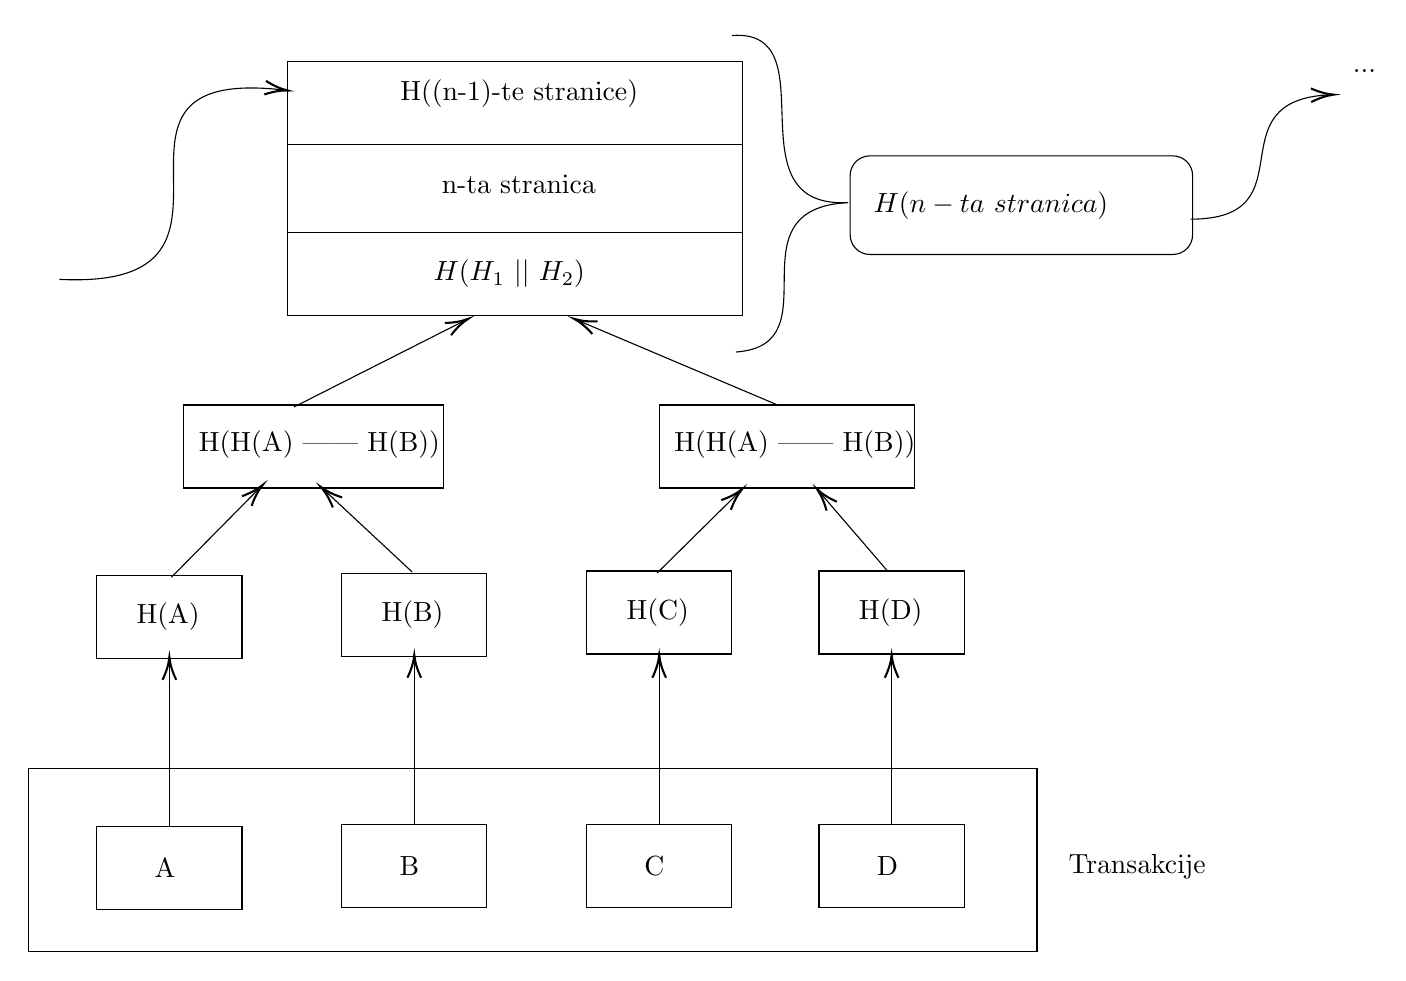
\begin{tikzpicture}[x=0.75pt,y=0.75pt,yscale=-1,xscale=1]
%uncomment if require: \path (0,497); %set diagram left start at 0, and has height of 497

%Shape: Rectangle [id:dp4321179914766464] 
\draw   (6,386) -- (492,386) -- (492,474.5) -- (6,474.5) -- cycle ;
%Shape: Rectangle [id:dp8872489473788213] 
\draw   (157,413) -- (227,413) -- (227,453) -- (157,453) -- cycle ;
%Straight Lines [id:da6623694321503638] 
\draw    (192,413) -- (192,333.5) ;
\draw [shift={(192,331.5)}, rotate = 450] [color={rgb, 255:red, 0; green, 0; blue, 0 }  ][line width=0.75]    (10.93,-3.29) .. controls (6.95,-1.4) and (3.31,-0.3) .. (0,0) .. controls (3.31,0.3) and (6.95,1.4) .. (10.93,3.29)   ;
%Shape: Rectangle [id:dp19081926795582194] 
\draw   (39,414) -- (109,414) -- (109,454) -- (39,454) -- cycle ;
%Straight Lines [id:da07351744030248808] 
\draw    (74,414) -- (74,334.5) ;
\draw [shift={(74,332.5)}, rotate = 450] [color={rgb, 255:red, 0; green, 0; blue, 0 }  ][line width=0.75]    (10.93,-3.29) .. controls (6.95,-1.4) and (3.31,-0.3) .. (0,0) .. controls (3.31,0.3) and (6.95,1.4) .. (10.93,3.29)   ;
%Shape: Rectangle [id:dp6447732440433431] 
\draw   (275,413) -- (345,413) -- (345,453) -- (275,453) -- cycle ;
%Straight Lines [id:da08996489921985373] 
\draw    (310,413) -- (310,333.5) ;
\draw [shift={(310,331.5)}, rotate = 450] [color={rgb, 255:red, 0; green, 0; blue, 0 }  ][line width=0.75]    (10.93,-3.29) .. controls (6.95,-1.4) and (3.31,-0.3) .. (0,0) .. controls (3.31,0.3) and (6.95,1.4) .. (10.93,3.29)   ;
%Shape: Rectangle [id:dp35045307677532056] 
\draw   (39,293) -- (109,293) -- (109,333) -- (39,333) -- cycle ;
%Shape: Rectangle [id:dp10554006421694595] 
\draw   (157,292) -- (227,292) -- (227,332) -- (157,332) -- cycle ;
%Shape: Rectangle [id:dp5131724308650354] 
\draw   (275,291) -- (345,291) -- (345,331) -- (275,331) -- cycle ;
%Shape: Rectangle [id:dp6283638134506683] 
\draw   (387,413) -- (457,413) -- (457,453) -- (387,453) -- cycle ;
%Straight Lines [id:da030731226630209663] 
\draw    (422,413) -- (422,333.5) ;
\draw [shift={(422,331.5)}, rotate = 450] [color={rgb, 255:red, 0; green, 0; blue, 0 }  ][line width=0.75]    (10.93,-3.29) .. controls (6.95,-1.4) and (3.31,-0.3) .. (0,0) .. controls (3.31,0.3) and (6.95,1.4) .. (10.93,3.29)   ;
%Shape: Rectangle [id:dp9520395935308572] 
\draw   (387,291) -- (457,291) -- (457,331) -- (387,331) -- cycle ;
%Shape: Rectangle [id:dp8077340163423831] 
\draw   (81,211) -- (206,211) -- (206,251) -- (81,251) -- cycle ;
%Straight Lines [id:da4393123411447112] 
\draw    (75,294) -- (117.59,250.92) ;
\draw [shift={(119,249.5)}, rotate = 494.68] [color={rgb, 255:red, 0; green, 0; blue, 0 }  ][line width=0.75]    (10.93,-3.29) .. controls (6.95,-1.4) and (3.31,-0.3) .. (0,0) .. controls (3.31,0.3) and (6.95,1.4) .. (10.93,3.29)   ;
%Straight Lines [id:da6905852604893123] 
\draw    (191,291.5) -- (148.46,251.86) ;
\draw [shift={(147,250.5)}, rotate = 402.98] [color={rgb, 255:red, 0; green, 0; blue, 0 }  ][line width=0.75]    (10.93,-3.29) .. controls (6.95,-1.4) and (3.31,-0.3) .. (0,0) .. controls (3.31,0.3) and (6.95,1.4) .. (10.93,3.29)   ;
%Shape: Rectangle [id:dp9330661027381227] 
\draw   (310,211) -- (433,211) -- (433,251) -- (310,251) -- cycle ;
%Straight Lines [id:da647758351674839] 
\draw    (309,292) -- (348.58,252.91) ;
\draw [shift={(350,251.5)}, rotate = 495.35] [color={rgb, 255:red, 0; green, 0; blue, 0 }  ][line width=0.75]    (10.93,-3.29) .. controls (6.95,-1.4) and (3.31,-0.3) .. (0,0) .. controls (3.31,0.3) and (6.95,1.4) .. (10.93,3.29)   ;
%Straight Lines [id:da48415803839754723] 
\draw    (420,291) -- (387.3,253.02) ;
\draw [shift={(386,251.5)}, rotate = 409.28] [color={rgb, 255:red, 0; green, 0; blue, 0 }  ][line width=0.75]    (10.93,-3.29) .. controls (6.95,-1.4) and (3.31,-0.3) .. (0,0) .. controls (3.31,0.3) and (6.95,1.4) .. (10.93,3.29)   ;
%Shape: Rectangle [id:dp16929651221601583] 
\draw   (131,128) -- (350,128) -- (350,168) -- (131,168) -- cycle ;
%Straight Lines [id:da6737546570402214] 
\draw    (134,212) -- (216.22,170.4) ;
\draw [shift={(218,169.5)}, rotate = 513.1600000000001] [color={rgb, 255:red, 0; green, 0; blue, 0 }  ][line width=0.75]    (10.93,-3.29) .. controls (6.95,-1.4) and (3.31,-0.3) .. (0,0) .. controls (3.31,0.3) and (6.95,1.4) .. (10.93,3.29)   ;
%Straight Lines [id:da5027553081138414] 
\draw    (367,211) -- (270.84,170.28) ;
\draw [shift={(269,169.5)}, rotate = 382.95] [color={rgb, 255:red, 0; green, 0; blue, 0 }  ][line width=0.75]    (10.93,-3.29) .. controls (6.95,-1.4) and (3.31,-0.3) .. (0,0) .. controls (3.31,0.3) and (6.95,1.4) .. (10.93,3.29)   ;
%Shape: Rectangle [id:dp5600508754383059] 
\draw   (131,45.5) -- (350,45.5) -- (350,168) -- (131,168) -- cycle ;
%Shape: Rectangle [id:dp41245370653393054] 
\draw   (131,45.5) -- (350,45.5) -- (350,85.5) -- (131,85.5) -- cycle ;
%Curve Lines [id:da0041357615969599415] 
\draw    (21,150.5) .. controls (131.45,155.97) and (21.11,46.6) .. (129.35,59.3) ;
\draw [shift={(131,59.5)}, rotate = 187.19] [color={rgb, 255:red, 0; green, 0; blue, 0 }  ][line width=0.75]    (10.93,-3.29) .. controls (6.95,-1.4) and (3.31,-0.3) .. (0,0) .. controls (3.31,0.3) and (6.95,1.4) .. (10.93,3.29)   ;
%Curve Lines [id:da26642107281708394] 
\draw    (566,121.5) .. controls (624.41,121.5) and (575.99,64.16) .. (633.23,61.56) ;
\draw [shift={(635,61.5)}, rotate = 538.5699999999999] [color={rgb, 255:red, 0; green, 0; blue, 0 }  ][line width=0.75]    (10.93,-3.29) .. controls (6.95,-1.4) and (3.31,-0.3) .. (0,0) .. controls (3.31,0.3) and (6.95,1.4) .. (10.93,3.29)   ;
%Rounded Rect [id:dp045619355532657946] 
\draw   (402,100.5) .. controls (402,95.25) and (406.25,91) .. (411.5,91) -- (557.5,91) .. controls (562.75,91) and (567,95.25) .. (567,100.5) -- (567,129) .. controls (567,134.25) and (562.75,138.5) .. (557.5,138.5) -- (411.5,138.5) .. controls (406.25,138.5) and (402,134.25) .. (402,129) -- cycle ;
%Curve Lines [id:da13309486554182137] 
\draw    (345,33) .. controls (393,29.5) and (343,116.5) .. (401,113.5) ;
%Curve Lines [id:da10324455292651535] 
\draw    (347,185.5) .. controls (395,182) and (343,116.5) .. (401,113.5) ;

% Text Node
\draw (192,433) node   [align=left] {\begin{minipage}[lt]{10.65pt}\setlength\topsep{0pt}
B
\end{minipage}};
% Text Node
\draw (74,434) node   [align=left] {\begin{minipage}[lt]{10.65pt}\setlength\topsep{0pt}
A
\end{minipage}};
% Text Node
\draw (310,433) node   [align=left] {\begin{minipage}[lt]{10.65pt}\setlength\topsep{0pt}
C
\end{minipage}};
% Text Node
\draw (57,305) node [anchor=north west][inner sep=0.75pt]   [align=left] {H(A)};
% Text Node
\draw (175,304) node [anchor=north west][inner sep=0.75pt]   [align=left] {H(B)};
% Text Node
\draw (293,303) node [anchor=north west][inner sep=0.75pt]   [align=left] {H(C)};
% Text Node
\draw (422,433) node   [align=left] {\begin{minipage}[lt]{10.65pt}\setlength\topsep{0pt}
D
\end{minipage}};
% Text Node
\draw (405,303) node [anchor=north west][inner sep=0.75pt]   [align=left] {H(D)};
% Text Node
\draw (87,222) node [anchor=north west][inner sep=0.75pt]   [align=left] {H(H(A) || H(B))};
% Text Node
\draw (316,222) node [anchor=north west][inner sep=0.75pt]   [align=left] {H(H(A) || H(B))};
% Text Node
\draw (200,140) node [anchor=north west][inner sep=0.75pt]    {$H( H_{1} \ ||\ H_{2})$};
% Text Node
\draw (204,99) node [anchor=north west][inner sep=0.75pt]   [align=left] {n-ta stranica};
% Text Node
\draw (184,53) node [anchor=north west][inner sep=0.75pt]   [align=left] {H((n-1)-te stranice)};
% Text Node
\draw (412,107) node [anchor=north west][inner sep=0.75pt]    {$H( n-ta\ stranica)$};
% Text Node
\draw (643,48) node [anchor=north west][inner sep=0.75pt]   [align=left] {...};
% Text Node
\draw (506,426) node [anchor=north west][inner sep=0.75pt]   [align=left] {Transakcije};


\end{tikzpicture}
    }%
    \caption{Skica uključivanja Merkleovog stabla u stranicu}
\end{figure}

\subsection{Stranica}
Stranica je struktura podataka koja ima rezervirana specijalna polja za sljedeće informacije:
\begin{itemize}
    \item verziju protokola
    \item \textbf{sažetak prethodne stranice}
    \item sažetak korijena Merkleovog stabla transakcija
    \item oznaku vremena nastanka bloka u UNIX formatu
    \item izračunatu cjelobrojnu vrijednost $ N $ težine mreže
    \item pronađeni slučajni broj koji sadržava $ N $ vodećih nul-bitova
    \item varijabilni cijeli broj $ T $
    \item polje od $ T $ transakcija (najčešće veličine 1-2 MB)
\end{itemize}

\subsection{Transakcija}
Transakcije u Bitcoin mreži organizirane su u takozvane nepotrošene izlaze (engl. \textit{UTXO - Unspent Transaction Output}) koji se sastoje od varijabilnog broja ulaza (\textit{TxIn}) i 2 izlaza (\textit{TxOut}). Razlog za dva izlaza jest slanje samo dijela iznosa na nečiju adresu i usmjeravanje ostatka natrag na vlastitu adresu. Broj ulaza varira jer možemo primiti više iznosa s više adresa.

\label{block_reward}
Postoji posebna vrsta transakcija zvana baza novca (engl. \textit{coinbase}) koje nemaju ulaze. Njih rudar dodaje sa svojom adresom kao odredišnom jer prema specifikaciji Bitcoina on to smije napraviti i ostatak mreže će prihvatiti takav blok kao važeći. To se naziva nagrada za stranicu (engl. \textit{block reward}) te se iznos prepolavlja svakih 210.000 stranica ($\approx$ \text{4 godine}).

% =========================

\subsection{Potvrđivanje transakcija digitalnim potpisima}
Bitcoin, nesumnjivo vodeća kriptovaluta današnjice, jedan je od jednostavnijih primjera implementacije protokola za digitalni novac temeljen na ideji lanca stranica. Objasnit ćemo ukratko ideju rada Bitcoina i njegova ograničenja. Čvorovi Bitcoin mreže postižu suglasje takozvanim rudarenjem što je zapravo uzastopno ponavljanje operacija izračunavanja SHA-256 sažetka stranice (engl. \textit{ledger}) konkateniranog s nekom vrijednosti koju rudar mora pronaći kako bi zadovoljio zahtjev mreže - a to je da konačni sažetak ima prefiks od $N$ nul-bitova. Broj N zove se težina (engl. \textit{difficulty}) te je on direktno povezan s vjerojatnošću pronalaženja takvog sažetka. To se radi kako bi čvor koji uspješno pronađe taj sažetak mogao dokazati ostatku mreže da je on (u prosjeku) uložio vrijeme proporcionalno broju zahtjevanih prefiks nula. Ostatak mreže mu mora vjerovati jer ne postoji prečica kojom bi se predvidjela vrijednost funkcije sažetka bez da ju zapravo provedemo. Integritet Bitcoin lanca oslanja se na uvjerenje da je SHA-256 kriptografski sigurna funkcija sažetka. Opisat ćemo u nekoliko koraka proces kojim bi zamišljeni aktori Alice i Bob proveli transakciju u Bitcoin mreži:

\begin{enumerate}
    \interfootnotelinepenalty=10000
	\item Alice i Bob izgeneriraju kriptografske ključeve shemom digitalnog potpisa.
	\item Alice izradi transakciju u kojoj navodi da Bobu šalje određeni iznos novca. Alice zatim potpiše tu izjavu (engl. \textit{claim}) svojim tajnim ključem te ju objavi u mrežu

	\item Objava transakcije mreži je anonimna. Iako se koristi TCP, vrlo je teško otkriti pravo izvorište transakcije. Anonimizacija se postiže tzv. \textit{gossip protokolom}. Kada se primi ispravna poruka, svaki ju čvor prosljeđuje susjednim čvorovima, a ti čvorovi svojim susjedima itd.
	\item Rudari dodaju Alicinu transakciju na listu nepotvrđenih transakcija \footnotemark.
	\footnotetext{\textit{Unconfirmed transaction pool} je bazen (prioritetni red nepotvrđenih transakcija koje se trebaju obraditi). On je sortiran tako da rudar iz njega uzima transakcije koje njemu donose najveći profit te ih validira i dodaje na popis u sljedeću stranicu koju treba izrudariti.}
	
	\item Rudar će iz prioritetnog reda sortiranog po veličini naknade za svoju uslugu\footnotemark uzimati transakcije, provjeriti ispravnost potpisa te njihovu odgovaraju li oni zapisima u bazi povijesti lanca stranica.
	\footnotetext{\textit{Transaction fee} je mali iznos koji plaćamo rudaru za njegovu uslugu potvrđivanja naše transakcije kako bi ga motivirali da uključi zapis o našoj transakciji u sljedeću stranicu koju će izrudariti.}
	
	\item Ako je transakcija ispravna, rudar dodaje transakciju na popis u sljedeću stranicu u lancu koju treba \say{izrudariti}.
	\item Važeće transakcije spremaju se u binarno stablo gdje je roditeljski sažetak jednak sažetku oba sažetka djece\footnotemark. Takva struktura podataka olakšava izračunavanje SHA sažetka bez da moramo trošiti vrijeme na ponovno izračunavanje svih starih SHA-256 sažetaka prijašnjih transakcija u stablu koje stalno raste. Pri dodavanju novih transakcija moramo samo ažurirati jednu granu u tom stablu koja vodi do korijenskog sažetka koji u konačnici završava u opisniku stranice zajedno sa zaglavljem stranice, i odredišnom adresom rudara \footnotetext{\textit{Merkle tree} ili u Ethereum mreži \textit{Patricia (prefix) trie} je struktura podataka koja se koristi za pohranjivanje valjanih tekućih transakcija (više u \ref{merkle}).}
	
	\item U stranici postoji mjesto rezervirano za poseban broj kojeg rudar traži grubom silom tako da sažetak opisnika stranice ima svojstvo koje zahtijeva mreža ($N$ vodećih nul-bitova)\footnotemark.
	\footnotetext{\textit{Difficulty} ili težina mreže je broj vodećih 0-bitova koje sažetak lanca mora sadržavati}
	
	\item Uslijed pronalaženja sažetka s odgovarjuće težine, on objavljuje svoju stranicu susjednim čvorovima i na taj se način nova stranica propagira kroz mrežu. Svi čvorovi preuzimaju novu stranicu, prestaju sa traženjem svojeg \textit{noncea} te ponovno grade novu stranicu na upravo primljenoj stranici.
	\item Čvorovi koji još nisu čuli za novu stranicu, nastavljaju se natjecati s njom. Ukoliko dođe do istovremenog rudarenja više jednakovrijednih stranica na različitim računalima, onaj koji se uspije propagirati na više čvorova ima veće izglede da će izrudariti i sljedeću stranicu zasnovanu na toj stranici te time 'pobijediti'\footnotemark
	\footnotetext{\textit{Orphaned block} je stranica koja je odbačena jer je započela kraću granu u lancu, a prema suglasju mreže, uvijek moramo graditi na najduljem lancu jer je on autoritativan te prikazuje stvarno stanje mreže. Transakcije na odbačenim stranicama postaju nevažeće. To je jedan od razloga zašto se savjetuje da se pričeka nekoliko blokova prije nego što se vjeruje posljednjoj izrudarenoj stranici}
	\footnotemark.
	\footnotetext{\textit{Forking} ili račvanje je trenutak kada se još ne zna pravo stanje mreže zbog dvije stranice nastale u bliskom vremenskom okviru. To se relativno brzo razrješava rudarenjem već sljedeće stranice nakon jedne od njih}
	Prosječno vrijeme potrebno za nastanak nove stranice u Bitcoin mreži je 10 minuta (dok neki lanci stranica poput Ethereuma imaju znatno kraće vrijeme od 14 sekundi). Stoga je privremeno račvanje češća pojava u Ethereum mreži.
\end{enumerate}

\subsection{Vrijeme stranice}
Pojam vrijeme stranice odnosi se na prosječno vrijeme koje protekne između rudarenja dvije uzastopne stranice u lancu. Bitcoin ima samo-podesivi mehanizam ugrađen u protokol koji brine da prosječno vrijeme za pronalaženje sažetka sljedeće stranice bude oko 10 minuta. Međutim, novi čvorovi nastaju u mreži, a neki postojeći se gase te stoga ukupna komputacijska snaga doživljava stalne fluktuacije. Rješenje za taj problem je da se broj zahtijevanih vodećih nul-bitova u bloku prilagođava obrnuto proporcionalno prosječnom vremenu mreže svakih 2016 stranica (što je okvirno 2 tjedna). Svaki rudar taj broj može nezavisno izračunati te prilagoditi svoj ciljani broj vodećih nul-bitova koje traži. Na taj je način osigurano približno konstantno vrijeme stranice.

\section{Suglasje}
Prijenos valute u Bitcoin mreži provodi se kroz takozvane nepotrošene izlaze transakcija\footnotemark. Svaki nepotrošeni izlaz transakcija asociran je s jednim vlasnikom (kriptografskim javnim ključem) te ga može samo vlasnik odgovarajućeg privatnog ključa poslati na neku drugu adresu. Prilikom toga, nepotrošeni izlaz može biti raspoređen na više odredišta. Stoga, ako pošiljatelj ne želi poslati cijeli iznos nepotrošenog izlaza transakcije, svoju adresu mora navesti kao odredišnu za ostatak iznosa koji nije poslan primatelju.
\footnotetext{\textit{Unspent Transaction Output} (UTXO) je zapis koji uz sebe ima asocirane ulaze odnosno količine uplaćenog novca s jedne ili više adresa te dva izlaza koji određuju odredišne adrese. Dva izlaza služe slanju samo dijela sredstava na neku drugu adresu a ostatak usmjeriti natrag na vlastitu. Skup svih nepotrošenih izlaza transakcija je valuta u cirkulaciji i njega prati svaki rudar u mreži.}

Rudari moraju imati bazu podataka nepotrošenih izlaza transakcija te pri upitima za dodavanje novih transakcija na stranicu, čvorovi im uz strukturu transakcije moraju poslati i svoj javni ključ kako bi oni mogli provjeriti njezinu ispravnost \footnotemark. Službena propozicija Bitcoina ne specificira implementaciju takvih baza podataka, no teži se korištenju što bolje optimiziranih struktura podataka (npr. indeksiranja) lanca kako bi rudari ostali kompetitivni s ostatkom mreže uz što manje nepotrebnog računanja. Također postoje i čvorovi koji nude samo uslugu pretraživanja baze ili ogledala (engl. \textit{mirroring}) te čuvaju povijest svih provedenih transakcija u mreži. Primjerice, najpopularnija implementacija baze podataka za Bitcoin čvor koristi LevelDB bazu podataka koja nudi brzi pristup disku u strukturi polja raspršenog adresiranja.
\footnotetext{ Takozvani \textit{Full-node} je čvor koji u memoriji čuva skup nepotrošenih izlaza transakcija u svrhu validiranja ispravnosti budućih transakcija, čuvanje javnih ključeva drugih korisnika za provjeravanje }


\subsection{Dokaz rada}
Dokaz rada je osmišljen kako bi se zlonamjernim čvorovima onemogućilo razglašavanje pogrešne informacije o stanju mreže (primjer: razglase da imaju više Bitcoina u svom vlasništvu ili više puta potroše iste Bitcoine koje posjeduju). Dokaz rada fizički onemogućava takve pokušaje prevare zato što bi za takvo što napadač morao imati većinu računalne snage u mreži što svakako nije moguće. Međutim centralizacija je i dalje velik problem u Bitcoinu jer kompanije s najjačom opremom imaju najveće izglede za pronaći sažetak sljedećeg bloka \cite{9160462}. Poticaj rudarima da obavljaju taj zahtjevan posao je činjenica da će prema dogovoru specifikacije biti nagrađeni određenim iznosom kriptovalute\footnotemark
\footnotetext{\textit{Block reward} --- vidi \ref{block_reward}}
Kako bi rudari imali interesa uopće uključivati transakcije i graditi Merkleova stabla, biti će dodatno nagrađeni i od svake obrađene transakcije prema informaciji koju je izdavatelj odredio. Zato su transakcije organizirane u prioritetni red --- rudarima se više isplati prvo obrađivati transakcije sa višom naknadom te će one prije biti potvrđene. Moguć je scenarij da transakcije nikada ne budu uključene na popis stranice jer naprosto imaju prenisku naknadu, a ispred nje u red prevelikom brzinom dolaze nove transakcije. Međutim, ne možemo biti sigurni da nikada neće biti potvrđena transakcija sa niskom naknadom. Mehanizam otkazivanja transakcija ne postoji te je velik rizik ostaviti ju u prioritetnom redu rudara. Novac se može \say{spasiti} dvostrukom potrošnjom\footnotemark na drugi vlastiti račun uz znatno višu naknadu kako bi bila potvrđena prije navedene \textit{"spore"} transakcije.
\footnotetext{\textit{Double spending} je pojava kada napravimo transakciju (ili sumu transakcija) većeg iznosa no što posjedujemo. Nakon validiranja transakcija za koje imamo dovoljan iznos novaca, doći će na red naša stara transakcija te verifikacija neće uspijeti jer je \textit{TxOut} već potrošen. Rudari takve upite odbacuju.}

\subsubsection{Negativne strane dokaza rada}
U teoretskom napadu\footnotemark od 51 \% snage radi se upravo o tome da grupa koordiniranih zlonamjernih čvorova može blokirati ostale rudare od natjecanja za sljedeću stranicu. Kada bi se našla takva hipotetska organizacija, ništa ju ne bi moglo zaustaviti i ne postoji pravi način da se mreža zaštiti od takvog napada. Oni bi mogli generirati prazne stranice (što je potpuno legalno) te ih periodički propuštati ostatku mreže kako bi odustali od svojeg uzaludnog rada. Sav rad poštenih čvorova u mreži bio bi uzaludan i stranice bi bile važeće i prazne. Ovaj se napad najčešće zanemaruje zbog neizglednosti da će jedna organizacija ikad imati procesorsku većinu. Međutim, statistike pokazuju drugačije - distribucija računalne snage između koordiniranih rudarskih bazena vrlo je segregirana i postoji stvarna prijetnja od ovakvog napada. Mreža nije toliko decentralizirana koliko je bilo planirano. Uzrok takve podjele u računalnoj snazi leži u specijaliziranom sklopovlju koje koristi sklopove (FPGA, ASIC) za računanje SHA-256 sažetaka nekoliko redova veličine brže no što to mogu grafičke kartice u klasičnom računalu. SHA-256 je bio dizajniran da bude brz jer mu primarna namijena nije bila osiguravanje lanca stranica.

U novijim se lancima stranica teži korištenju kriptografskih funkcija sažetaka za koje je vrlo teško napraviti efikasno specijalizirano sklopovlje koje bi bilo značajno bolje od računala opće namjene. Kao primjer takve kriptografske funkcije valja spomenuti familiju Keccak (NIST-ov SHA-3 standard) koji je baziran na spužvastoj konstrukciji koje i vrlo ga je teško paralelizirati specijaliziranim sklopovljem (vrlo niska prednost nad računalima opće namijene). (TODO!!!)

Također, mreže koje koriste dokaz rada imaju \textbf{problem skaliranja}. Naime, distribuirana baza podataka ograničena je na propusnost pisanja jednaku prosječnom čvoru. Kako bi lanac stranica bio izvediv kao sustav elektroničkog novca na globalnoj razini, trebao bi imati vrlo visoku propusnost pri obradi transakcija.

\subsection{Dokaz uloga}
Zbog niske ekonomičnosti dokaza rada, velikog opterećenja računalnih sustava, a posljedično i iznimno velike potrošnje električne energije, javila se nova metoda postizanja suglasja u mrežama bez dokaza rada: dokaz uloga. Idejno radi tako da se čvorovi validatori u mreži kandidiraju te uz vjerojatnost proporcionalnu njihovom ulogu u pametnom ugovoru, bivaju izabrani da validiraju sljedeću stranicu i time dobivaju nagradu. Pri pokušajima varanja ili neispravnoj validaciji čvor bi trebao biti kažnjen prema suglasju mreže tako da mu se velik dio njegovog uloga oduzme što napade čini vrlo nepraktičnima. Sada se problem 51 \% računalne snage prebacuje na problem većine sredstava što lanac čini znatno decentraliziranijim i otpornijim.

Primjerice, \textit{Ouroboros} \cite{ouroboros} je protokol razvijen za potrebe dokaza uloga korišten u Cardano (ADA) kriptovaluti je kriptovaluta koja se od svog početka oslanja na ovakav način rada, a Ethereum (ETH) unatoč tome što se trenutno oslanja na dokaz rada, ima eksponencijalno povećanje težine svakih 100.000 stranica kako bi potaknuo što bržu tranziciju mreže na dokaz uloga. \cite{wood2014ethereum}.

Ovakvo suglasje ima znatno veću brzinu obrade transakcija jer nije potrebno trošiti vrijeme na rudarenje. On se javlja u kombinaciji sa idejom \textit{shardinga} koji dijeli mrežu na manje lance stranica što mreži daje veću propusnost zbog manje koordinacije između skupina lanaca. U takvim se lancima vodi briga o tome da skupovi transakcija koje pojedini \textit{shardovi} obrađuju budu disjunktni skupovi.

\subsubsection{Negativne strane dokaza uloga}
\newtheorem{problem}{Problem.}
\begin{problem}
Zamislimo sustav koji ima \textbf{n} komponenata, od kojih je \textbf{t} nepouzdano te se komunikacija odvija u dvosmjernim kanalima između dviju točaka. Koliko iznosi minimalni \textbf{n} kako bi se uspostavilo suglasje oko odgovora u sustavu?
\end{problem}

Leisle Lamport \cite{lamport1982the} je dokazao da je to moguće postići s $3 \cdot t + 1$ čvorova. Treba $\frac{2}{3}$ potvrda ispravnih čvorova kako bismo postigli suglasje.
Nekoliko je znanstvenika predložilo rješenje u sljedeća tri koraka:
\begin{itemize}
    \item \textit{pre-prepare}
    \begin{itemize}
        \item u ovoj fazi čvor koji je primio upit za promjenu stanja sustava šalje ostalim čvorovima  zahtjev za pripremanje promjene u sustavu
    \end{itemize}
    \item \textit{prepare}
    \begin{itemize}
        \item svi čvorovi koji su uspješno primili poruku za pripremu (a rade ispravno), šalju svim ostalim čvorovima poruku \textbf{prepare} te očekuju $t$ odgovora prije nego što pohrane promjene no što razglase da su pohranili promjene
    \end{itemize}
    \item \textit{commit}
    \begin{itemize}
        \item ako čvor s kojim je vanjski klijent inicirao komunikaciju uspješno primi $t$ \textbf{commit} poruka, smatrat će da je sustav uspješno izvršio \textit{"transakciju"}
    \end{itemize}
\end{itemize}

1999. simulirana je poboljšana praktična verzija (PBFT) \cite{castro1999practical} dokaza uloga koja rješava problem zagušenja mreže od previše razmijenjenih poruka između komponenata.
\section{Pametni ugovor}
Transakcija kao trajni zapis u Bitcoin mreži obična je informacija. Spomenuli smo također i naziv tvrdnja kao općenitiji naziv za podatke koje možemo zapisati u lanac stranica. Mreža Ethereum ima poopćeno shvaćanje pojma transakcije. Naime, moguće je da transakcije sadrže bilo kakve podatke te se na toj ideji zasniva pametan ugovor. Pametan ugovor je naziv za posebnu transakciju koja odredišnu adresu ima postavljenu na \textit{null} te u tijelu sadrži računalne instrukcije koje se mogu koristiti za izvršavanje algoritama u izoliranom okruženju \textit{Ethereum virtual machine}. To je znatno moćniji koncept od običnih trajnih zapisa koje nudi Bitcoin. Pametni se ugovori stvaraju u programskom jeziku Solidity te se prevode u \textit{bytecode} koji se zapisuje na lanac stranica \cite{wood2014ethereum}. Optimizacija kôda pri prevođenju je vrlo važna zbog visoke cijene usluge pohrane ugovora na lanac stranica. Programeri teže što manjem konačnom broju instrukcija. Sigurnosni problemi za rudare su eliminirani jer virtualna mašina nije integrirana sa sustavom domaćina (izvodi se u pješčaniku poput \textit{Javascripta} u \textit{web} pregledniku). Svaki ugovor ima svoju adresu i opcionalno definira vanjsko sučelje s kojim drugi aktori mreže mogu razmjenjivati poruke. Svi se ugovori nalaze u dijeljenom virtualnom adresnom prostoru mreže i njihovi implementacijski detalji javno su vidljivi. Rudari alociraju resurse na svojim računalima kako bi mogli izvoditi pametne ugovore u virtualnim strojevima. Beskonačne petlje i slične maliciozne pojave sprečavaju se tako da stvaratelj ugovora mora platiti cijenu proporcionalnu broju instrukcija koji bi se trebao izvesti u ugovoru (engl. \textit{gas limit}). Kada se potroši sav iznos, rudari prestaju izvoditi pametni ugovor.

Ogromna moć koju nam nude pametni ugovori je garancija budućih događaja na lancu. Oni su supstitucija za posrednička tijela poput javnog bilježništva u suvremenim sustavima. Nema potrebe za povjerenjem jer ugovor se ne može otkazati i njegovo je izvođenje predvidivo. Postoje dvije vrste novčanika u mreži: vanjski (engl. \textit{external account}) i ugovorni novčanici (engl. \textit{contract account}) kojima upravlja kod pametnog ugovora. Iz tog je razloga moguće napraviti autonomne aplikacije na pametnim ugovorima koje obavljaju složene zadatke raspodjele novca. Ethereum već ima veliki ekosustav distribuiranih aplikacija (engl. \textit{ĐApp}) izgrađenih na pametnim ugovorima. To je razlog zašto se češće koristi naziv platforma umjesto kriptovalute.

% Premijestil sam ovo tu jer objašnjavam od jednostavnihih koncepti prema složenijima.
\section{Pogreške (popraviti)}
Čvorovi mreže moraju biti u suglasju oko stanja sustava kako bi mogli donositi odluke o svojim budućim akcijama. Dakle, moraju svi dijeliti isti lanac stranica. To se postiže odbacivanjem svih drugih lanaca osim autoritativnog. Odluka o tome koji je lanac autoritativan donosi se na temelju većine računalne moći iz čega sljedi i najdulji lanac. Ako u bilo kojem trenutku nastanu dvije nove stranice te se propagiraju mrežom (to se naziva račvanje lanca --- \textit{forking}), jedna od njih će imati većinu rudarske snage. Prije no što se ispostavi koja je ispravna, one su jednakovrijedne i upravo zbog toga se privremeno ne vjeruje posljednjoj stranici u lancu. Vjerojatnost za takvu neizvjesnost u lancu je vrlo niska te opada eksponencijalnom brzinom ukoliko napadač posjeduje manjinu snage u mreži \cite{nakamoto2012bitcoin}. Račvanje u lancima stranica može se dogoditi i promjenom u protokolu te čvorovi koji naprave tranziciju na novu verziju mogu završiti na odvojenom lancu koji efektivno postaje nova kriptovaluta. Taj se proces naziva tvrdo račvanje (engl. \textit{hard fork}) i dogodio se primjerice između Bitcoina i Bitcoin Classic.

% =========================
\chapter{Simulacija postizanja suglasja}

U ovom ćemo poglavlju objasniti izradu programske podrške za simulaciju postizanja konsenzusa u lancu stranica u mreži s više sudionika. Suglasje protokola bit će da je najdulji ispravni lanac autoritativan.

\section{Opis}
Implementacija je ostvarena u programskim jezicima Python i Javascript. Sastoji se od dva dijela:
\begin{enumerate}
    \item \textit{Backenda} čvora koji je zapravo poslužitelj s kojim komuniciramo HTTP protokolom preko REST metoda. Poslužitelj je napisan u radnom okviru Flask. Aplikacija brine o generiranju ključeva za čvor i njihovog korištenja kod potpisivanja podataka. Za ostvarenje spremišta ključeva, korištene su kriptografske primitive iz knjižnice PyCryptodome.
\end{enumerate}
Drugi dio implementacije sastoji se od \textit{frontend} klijenta kojemu pristupamo kroz \textit{web} preglednik. Naravno, korišten je programski jezik Javascript bez dodatnih knjižnica. Korišten je standardni asinkroni API zasnovan na obećanjima i \texttt{fetch} upitima koji će pozivati Flask \textit{backend} našeg čvora. Zajedno ta dva dijela čine jedan čvor u mreži. Programsku podršku možemo instalirati na više računala te simulirati njihovu međusobnu interakciju: postizanje suglasja i vršenje transakcija. Serijalizacijski format korišten za komunikaciju je JSON i sve poruke u sustavu prenose se u tekstualnom obliku (za razliku od Bitcoinovog binarnog protokola).

\section{Izrada transakcija}

\subsection{Adrese}
Adrese digitalnih novčanika u ovoj se simulaciji izračunavaju kao SHA-256 sažetak javnog ključa čvora nakon njihove serijalizacije u PEM format (ASCII kodiranu DER strukturu javnog ključa). Adresa kao sažetak javnog ključa uobičajena je praksa u popularnim implementacijama lanca stranica.

\subsection{Struktura transakcije}
Transakciju na vrlo jednostavan način stvaramo u \textit{web} pregledniku tako da unesemo odredišnu adresu i iznos koji želimo poslati na tu adresu. Tijelo upita u implementaciji formatirano je na sljedeći način:
\begin{minted}[obeytabs=true,tabsize=4,frame=single,framesep=10pt]{json}
{
	"data": {
		"amount": 35,
		"block_index": 5,
		"dst": "<heksadekadska_adresa_pošiljatelja>",
		"src": "<heksadekadska_adresa_primatelja>"
	},
	"pub_key": "-----BEGIN PUBLIC KEY-----...",
	"signature": "<heksadekadski_potpis_pošiljatelja>"
}
\end{minted}

Slanje čvoru (poslužitelju/rudaru) upit za stavljanje nove transakcije u bazen nepotvrđenih transakcija te njihova konačna potvrda. Poslužitelj će provodi striktnu validaciju kako bi utvrdio je li transakcija ispravno strukturirana:

\begin{enumerate}
	\item mora sadržavati sva očekivana polja
	\item mora biti jedinstvena (provjerava se kako nebi došlo do malicioznog \textit{replayja} valjanih transakcija)
	\item mora imati valjani digitalni potpis (korištena je shema iz specifikacije FIPS-186-3)
	\item sažetak javnog ključa mora odgovarati izvorišnoj adresi
	\item provjeravaju se povijesne transakcije izvorišne adrese da se ustvrdi ima li dovoljno sredstava da obavi transakciju koju želi
\end{enumerate}

\section{Implementacija dokaza rada}
U svrhu pojednostavljenja sustava, nije implementiran mehanizam adaptivne težine mreže već je postavljena konstantna težina od jednog vodećeg nul-okteta. Rudar inkrementalno traži broj (engl. \textit{nonce}) koji sa sažetkom opisnika stranice zadovoljava taj kriterij. Vjerojatnost da je $k$-ti sažetak ispravan može se opisati običnom geometrijskom distribucijom:
$$
P(X=k) = (1 - p) ^ {k-1} \cdot p \qquad \qquad x=0,1,2,\ldots \, .
$$

Uz pretpostavku da je kodomena funkcije prefiksa prvog okteta sažetka uniformno distribuirana po polju $\{0,1\} ^{8}$, očekivani broj pokušaja prije nego što pogodimo ispravan broj iznosi:

\begin{equation} \label{eq1}
\begin{split}
E(X) &= \frac{1}{p} \qquad \qquad p = (\frac{1}{2}) ^ {8} = \frac{1}{256} \\
     &= 256
\end{split}
\end{equation}

Najvažniji isječak kôda dokaza rada može se opisati sljedećim pseudokodom:

\colorlet{gray}{gray!40}
\begin{minted}[obeytabs=true,tabsize=4,frame=single,framesep=10pt]{python}
last_nonce = last_block['nonce']
last_hash = self.hash(last_block)
nonce = 0
while True:
	start = time()
	if self.valid_nonce(last_nonce, nonce, last_hash):
		break
	else:
		nonce += 1
		end = time()
		to_sleep = 0.01 - (end - start)
		if to_sleep > 0:
		    sleep(to_sleep)

\end{minted}
Dodano je vremensko kašnjenje \textbf{isključivo} radi demonstracije da taj proces inače zna potrajati te zbog uloženog vremena i električne energije, rudar dobiva ugovorenu nagradu zajedno sa naknadama svake transakcije. Prosječno vrijeme stranice iznosi oko 2.5 sekunde.

\section{Implementacija sinkronizacije čvorova}

\section{REST sučelje aplikacije}
Kao što je spomenuto, aplikacija ima REST sučelje što znači da je moguće napraviti nezavisnog klijenta (čak i mobilnog) koji bi koristio čvor u mreži. Definirane su sljedeće metode za pregled i upravljanje stanjem čvora:

\begin{itemize}
	\item GET    /mine
	\begin{itemize}
		\item pokreće algoritam rudarenja sljedeće stranice koja će uključivati sve nepotvrđene transakcije iz reda čekanja
	\end{itemize}
	\item GET    /block\_id
	\begin{itemize}
		\item dohvaća ID trenutne stranice u lancu
	\end{itemize}
	\item GET    /txn
	\begin{itemize}
		\item dohvaća listu nepotvrđenih transakcija iz bazena transakcija
	\end{itemize}
	\item POST   /txn 
	\begin{itemize}
		\item dodaje novu transakciju u trenutni lanac ako je ispravno formatirana i logički valjana
		\item transakcija se zadaje kao tijelo upita u JSON formatu
	\end{itemize}
	\item GET    /pub\_key
	\begin{itemize}
		\item dohvaća javni ključ čvora
	\end{itemize}
	\item GET    /peer
	\begin{itemize}
		\item dohvaća listu spojenih susjednih čvorovima koji se kontaktiraju pri sinkronizaciji s mrežom
		\item u praktičnom lancu stranica ovaj je postupak automatiziran, no iz demonstracijskih razloga ručno se poziva na klik gumba u korisničkom sučelju
	\end{itemize}
	\item POST   /peer
	\begin{itemize}
		\item dodaje nove adrese u listu susjednih čvorova koje će koristiti za sinkronizaciju
	\end{itemize}
	\item DELETE /peer
	\begin{itemize}
		\item briše susjedni čvor iz liste ako postoji te ga više neće kontaktirati pri sinkronizaciji s mrežom
	\end{itemize}
	\item GET    /sync
	\begin{itemize}
		\item iterativno kontaktira sve susjedne čvorove kako bi dobio informacije o promjenama u mreži te, ako je netko izrudario novu stranicu na najduljem lancu, prihvaća njegov lanac kao autoritativan
	\end{itemize}
	\item POST   /sign
	\begin{itemize}
		\item privatnim ključem čvora digitalno potpisuje bilo kakav \textit{payload}
		\item koristi se za potpisivanje transakcije prije nego što se objavi u bazen
	\end{itemize}
	\item GET    /node\_id
	\begin{itemize}
		\item dohvaća identifikator trenutačnog čvora (adresu)
	\end{itemize}
	\item GET    /balance?address=<account\_address>
	\begin{itemize}
		\item izračunava količinu novca u vlasništvu neke adrese na temelju povijesti lanca
	\end{itemize}
	\item GET    /
	\begin{itemize}
		\item \textit{servira} statičku HTML \textit{web} stranicu klijenta
		\item čini pristupnu točku za internetske preglednike
	\end{itemize}
\end{itemize}

Pozivamo ih iz \textit{Javascripta} na \textit{frontendu} pomoću asinkronog \textit{fetch} sučelja. Nisu korištene dodatne vanjske knjižnice pri implementaciji. Na sličan se način mogu izgraditi i mobilni klijenti koji bi koristili rudarske čvorove u pozadini.

\section{Postizanje suglasja između više čvorova simulacije}
Suglasje se u simulaciji postiže prihvaćanjem najduljeg ispravnog lanca. Stoga, prilikom sinkronizacije čvor će poslati HTTP upit svim susjednim čvorovima da mu pošalju svoje stanje lanca. Valja napomenuti kako se u praksi mrežom šalju samo novonastale promjene u lancu prilikom sinkronizacije (npr. zadnjih $ N $ blokova glave lanca) radi brzine i manjeg zagušenja mreže redundantnim podacima. Ključni dio algoritma sinkronizacije prikazan je u isječku kôda ispod:

\begin{minted}[obeytabs=true,tabsize=4,frame=single,framesep=10pt]{python}
def synchronize_with_network(self):

    peers = self.nodes
    new_chain = None

    max_length = len(self.chain)

    for node in peers:
        response = None
        try:
            response = requests.get(f'http://{node}/chain')
            response.raise_for_status()
        except:
            print(f'Peer {node} didn\'t respond')
            pass

        if response and response.status_code == 200:
            length = response.json()['length']
            chain = response.json()['chain']

            if length > max_length and self.valid_chain(chain):
                max_length = length
                new_chain = chain

    if new_chain:
        self.chain = new_chain
        return True

    return False
\end{minted}

\chapter{Korištenje korisničkog sučelja}
Uporabu korisničkog sučelja demonstrirat ćemo na tri nezavisne instance programa. Svaki je pokrenut u svom Python okruženju slušajući upite na vlastitim vratima.

Pristupajući čvoru sa \textit{web} preglednika, prezentirani smo sa jednostavnom \textit{web} stranicom koja predstavlja naš novčanik. Pri svakoj interakciji sa stražnjim dijelom aplikacije, kontinuirano se osvježavaju informacije o našem računu.

\begin{figure}[H]
    \centering
    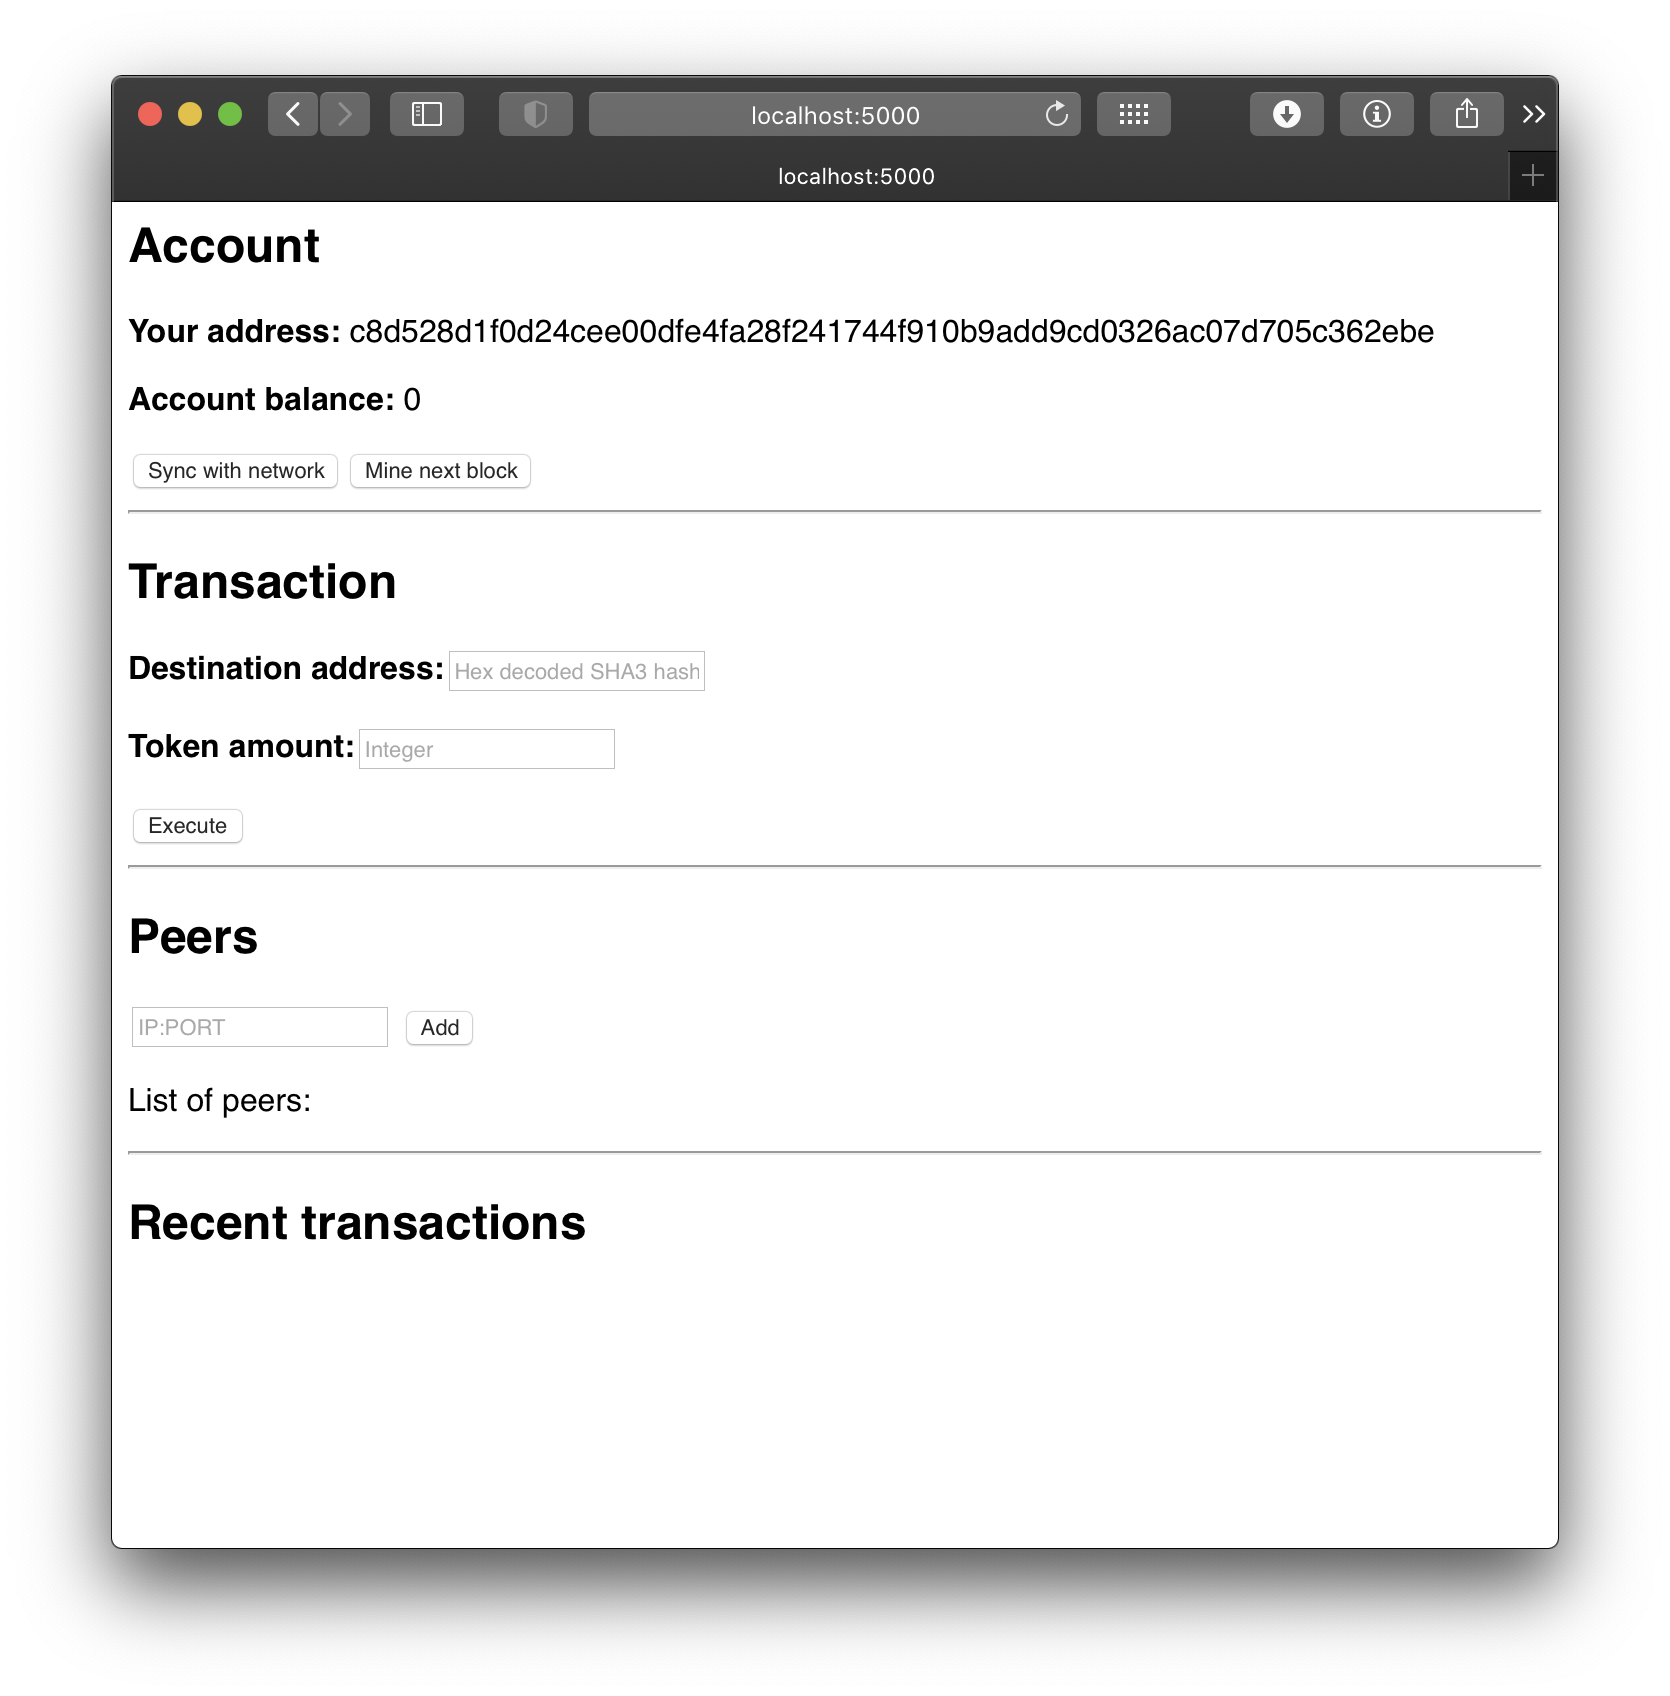
\includegraphics[width=\textwidth]{sucelje}
    \caption{Izgled korisničkog sučelja}
    \label{fig:sucelje}
\end{figure}

Klikom na gumb \keys{Mine}, šaljemo GET upit serveru čvora da pronađe \textit{nonce} za sljedeći blok koji ima pripremljen. Prva stranica koju pri pokretanju program automatski izrudari zove se \textit{genesis block}. Ona ima sažetak prethodnog bloka postavljen na \textit{null} te započinje novi lanac stranica.

\begin{figure}[H]
    \centering
    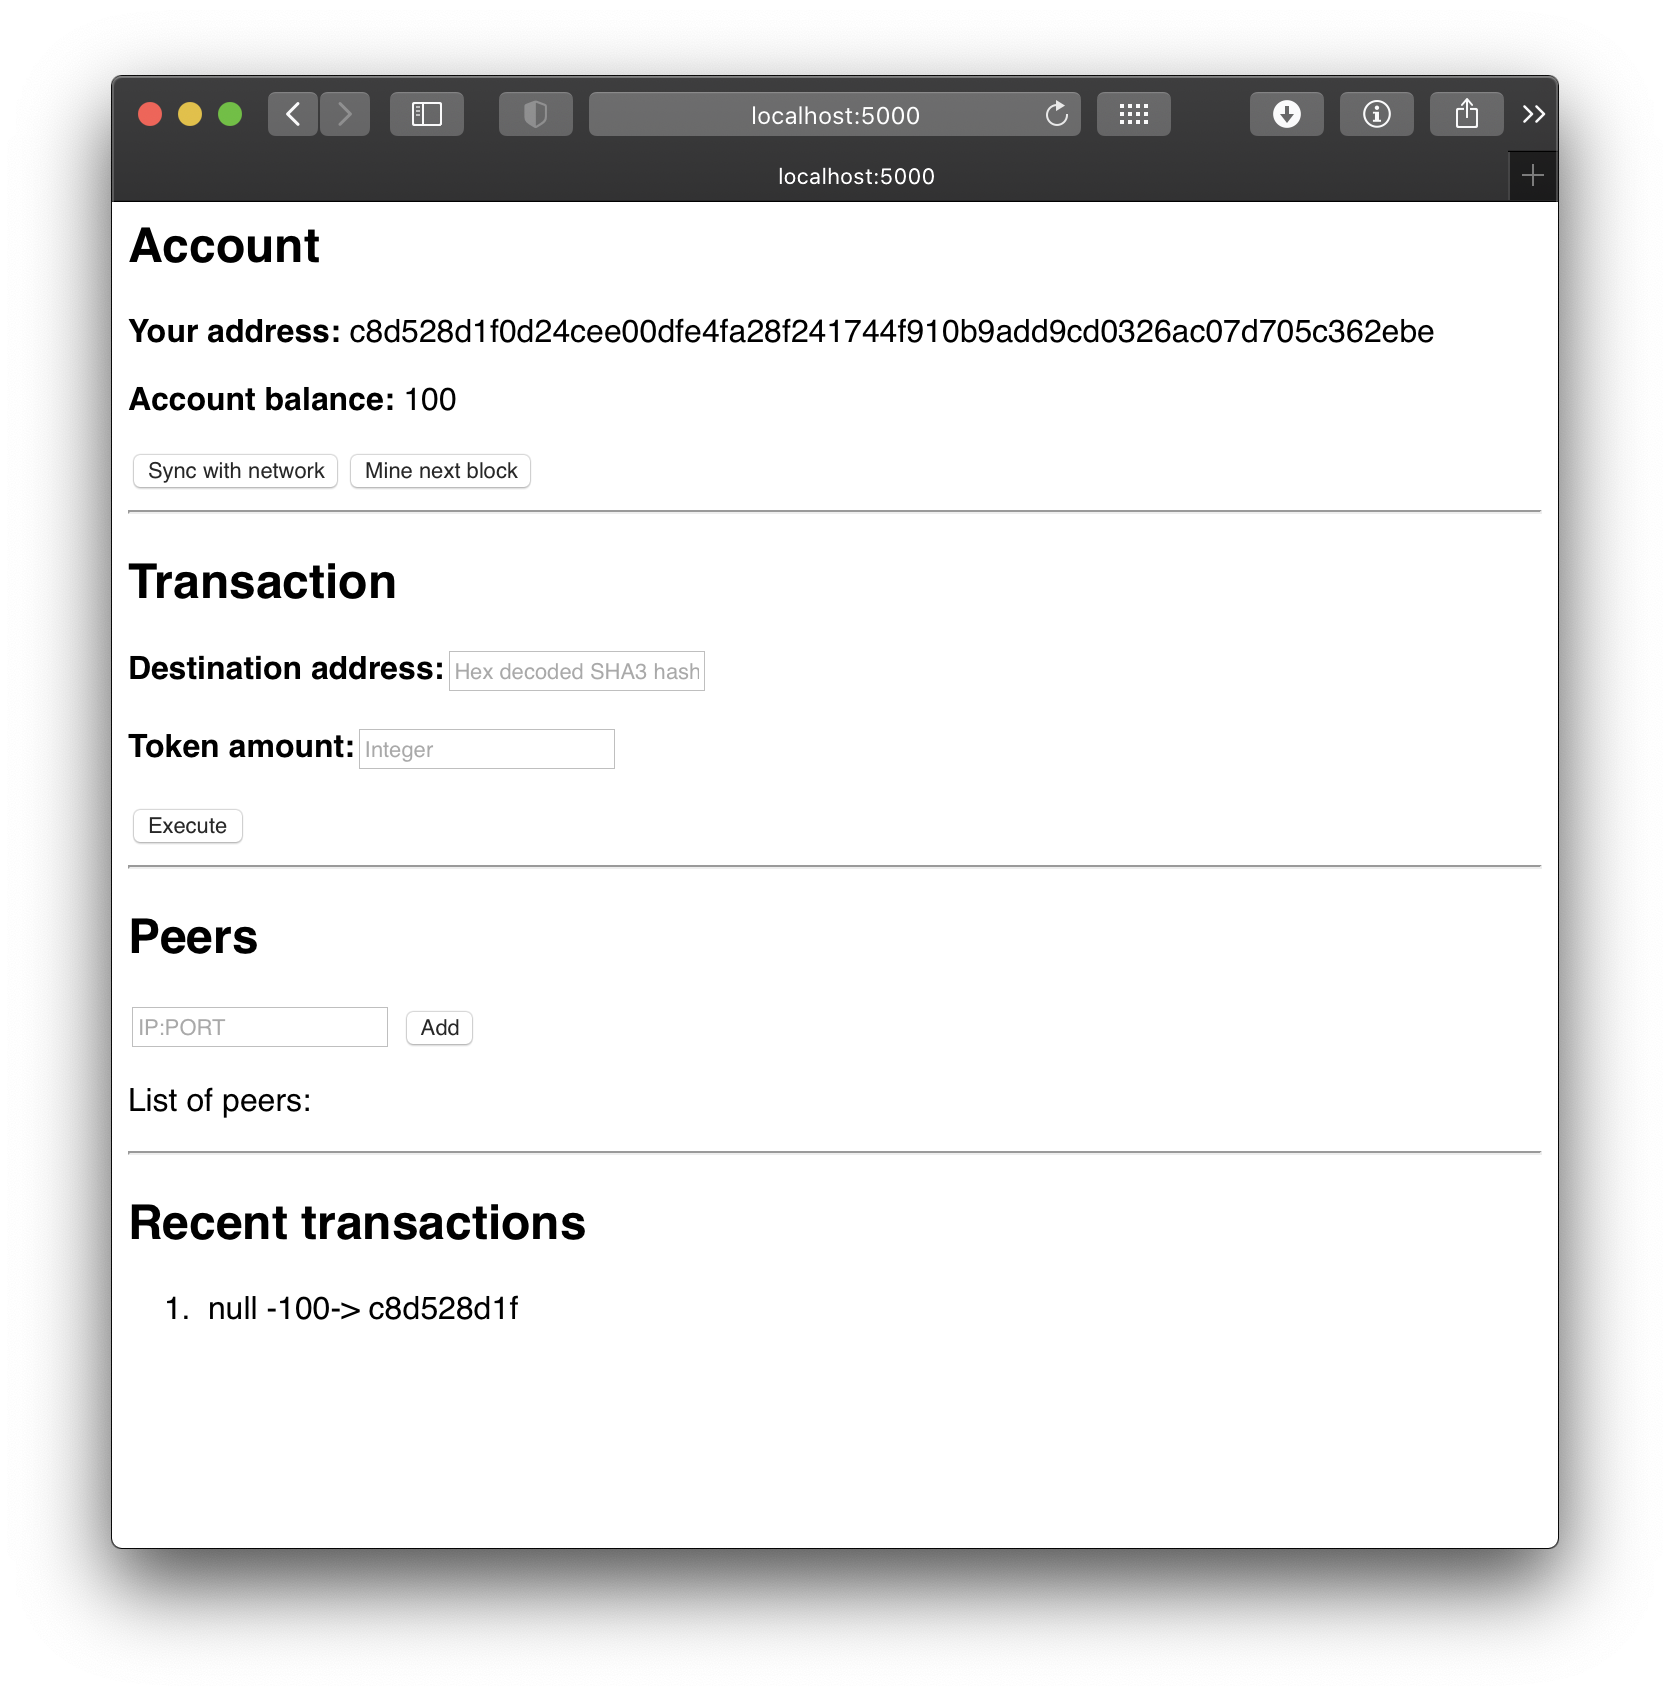
\includegraphics[width=\textwidth]{rudarenje}
    \caption{Rudarenje stranice}
    \label{fig:rudarenje}
\end{figure}

Kako bismo svog klijenta povezali sa susjednim čvorovima, upisujemo njihove IP adrese (ili imena domena) na listu \textit{peers}. Naš će čvor čuvati tu listu te pri pozivu \keys{Sync} će se pokušati sinkronizirati sa čvorovima šaljući im upite i uspoređujući lance.

\begin{figure}[H]
    \centering
    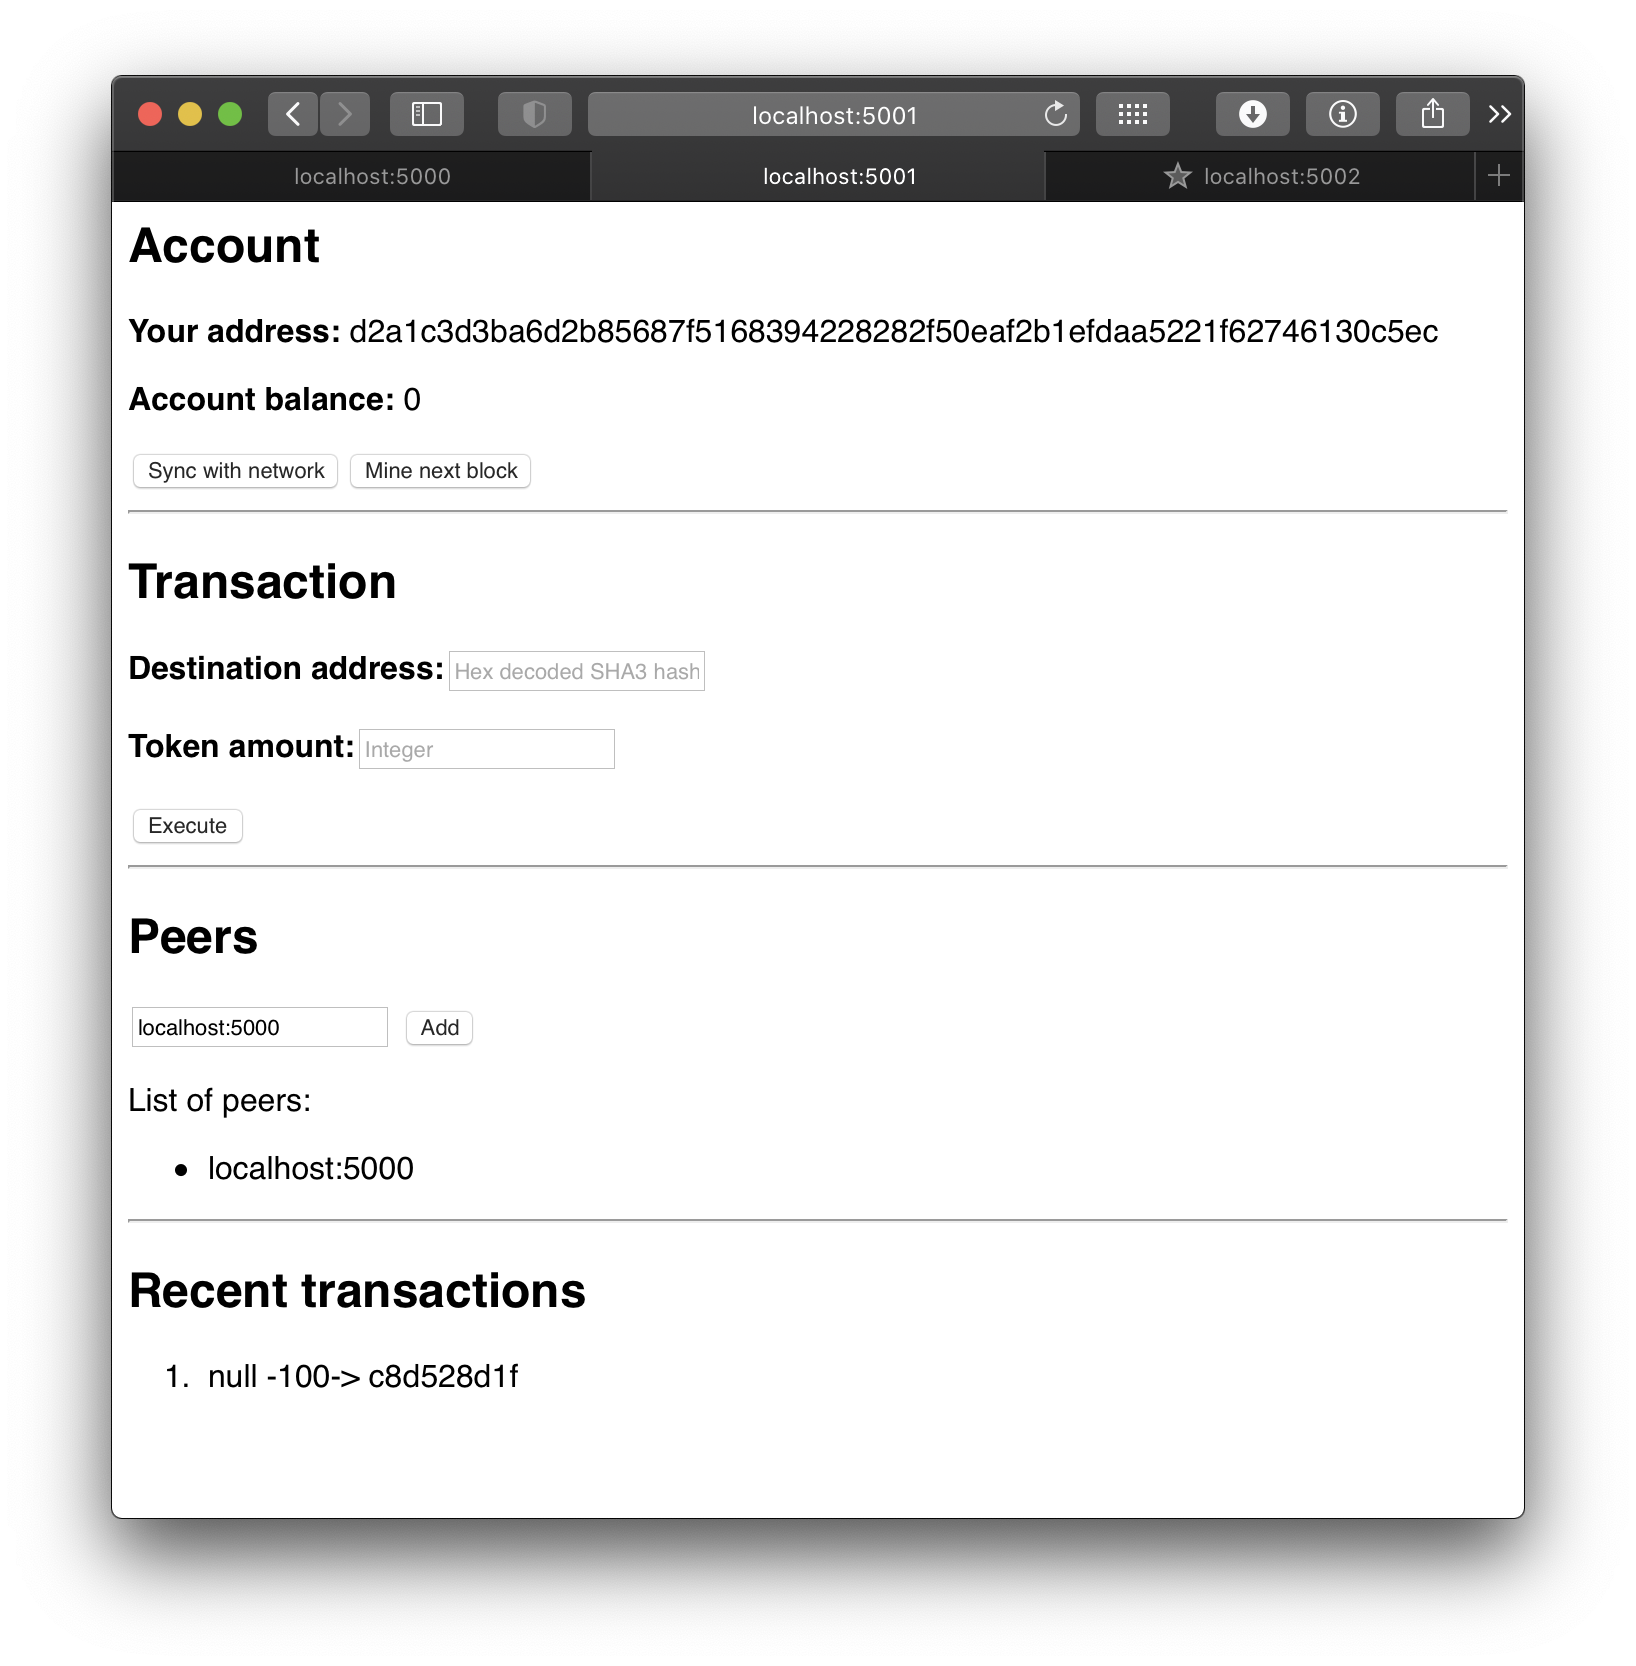
\includegraphics[width=\textwidth]{dodavanje_ip_adrese_susjeda.png}
    \caption{Dodavanje susjednih čvorova}
    \label{fig:dodaj_ip}
\end{figure}

Za provođenje nove transakcije, moramo samo navesti odredišnu adresu čvora, iznos koji želimo poslati tom čvoru i pritisnuti \keys{Execute}. Poslužitelj će provjeriti stanje lanca i format našeg upita i ukoliko prolazi sve provjere, dodati ga na listu još nepotvrđenih transakcija spremnih da budu izrudarene u sljedećoj stranici. Ponovnim klikom na \keys{Mine}, vidjet ćemo da se stanje našeg računa ažuriralo i transakcija je trajno zapisana na lanac stranica.

\begin{figure}[H]
    \centering
    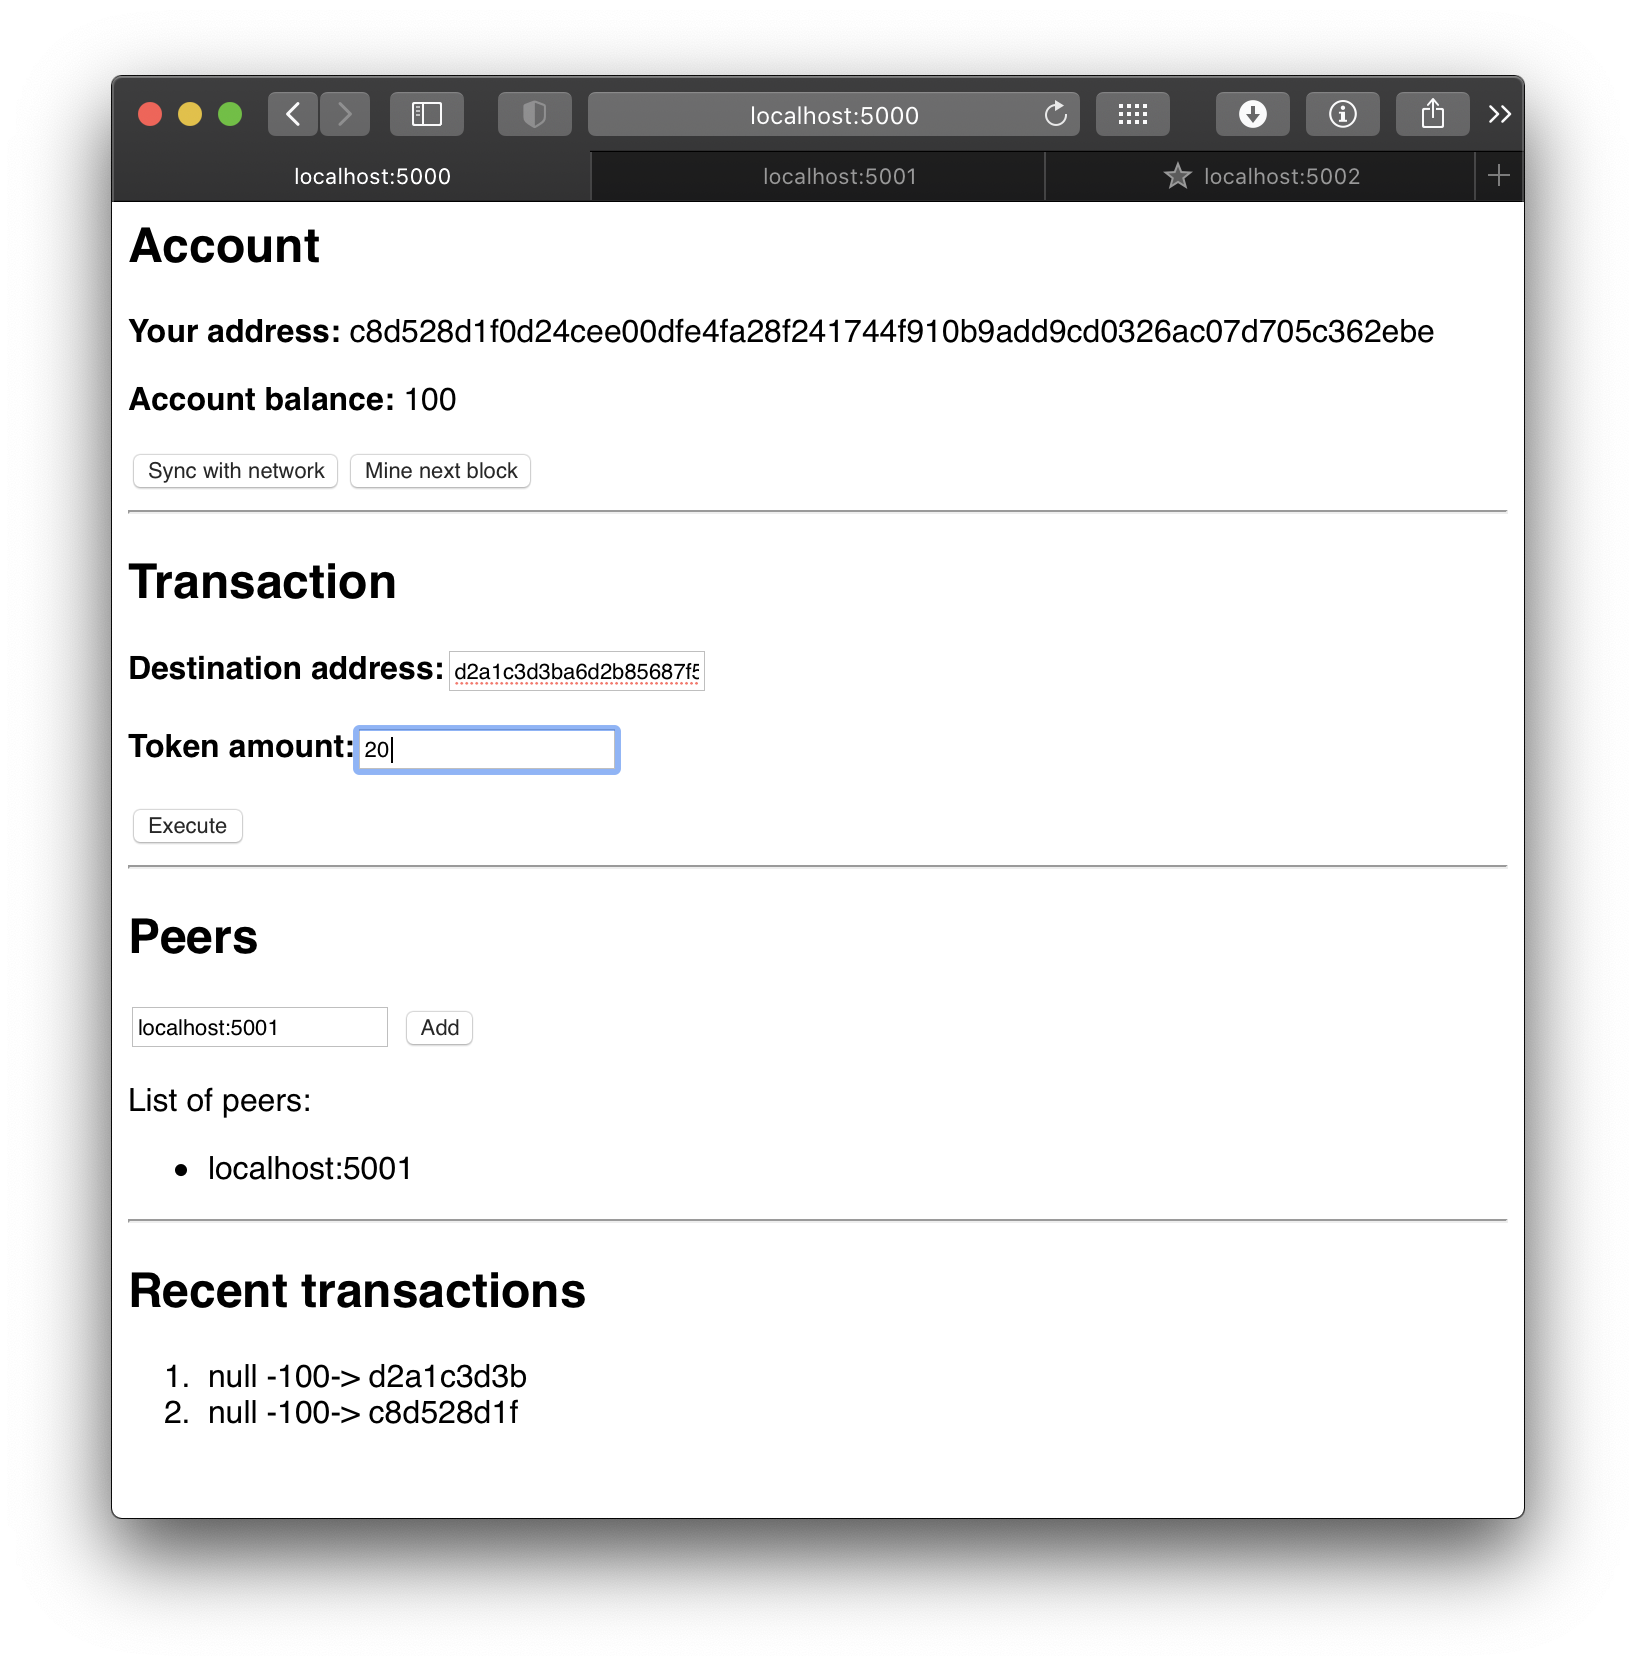
\includegraphics[width=\textwidth]{transakcija.png}
    \caption{Slanje novca}
    \label{fig:transakcija}
\end{figure}

Pogledajmo sada sustav iz perspektive primatelja. On još u svojem lancu nema nijedan blok jer ga nismo sinkronizirali s mrežom, no kada pritisnemo \keys{Sync}, povući će podatke sa prvog klijenta i osvježiti svoje stanje računa.

\begin{figure}[H]
    \centering
    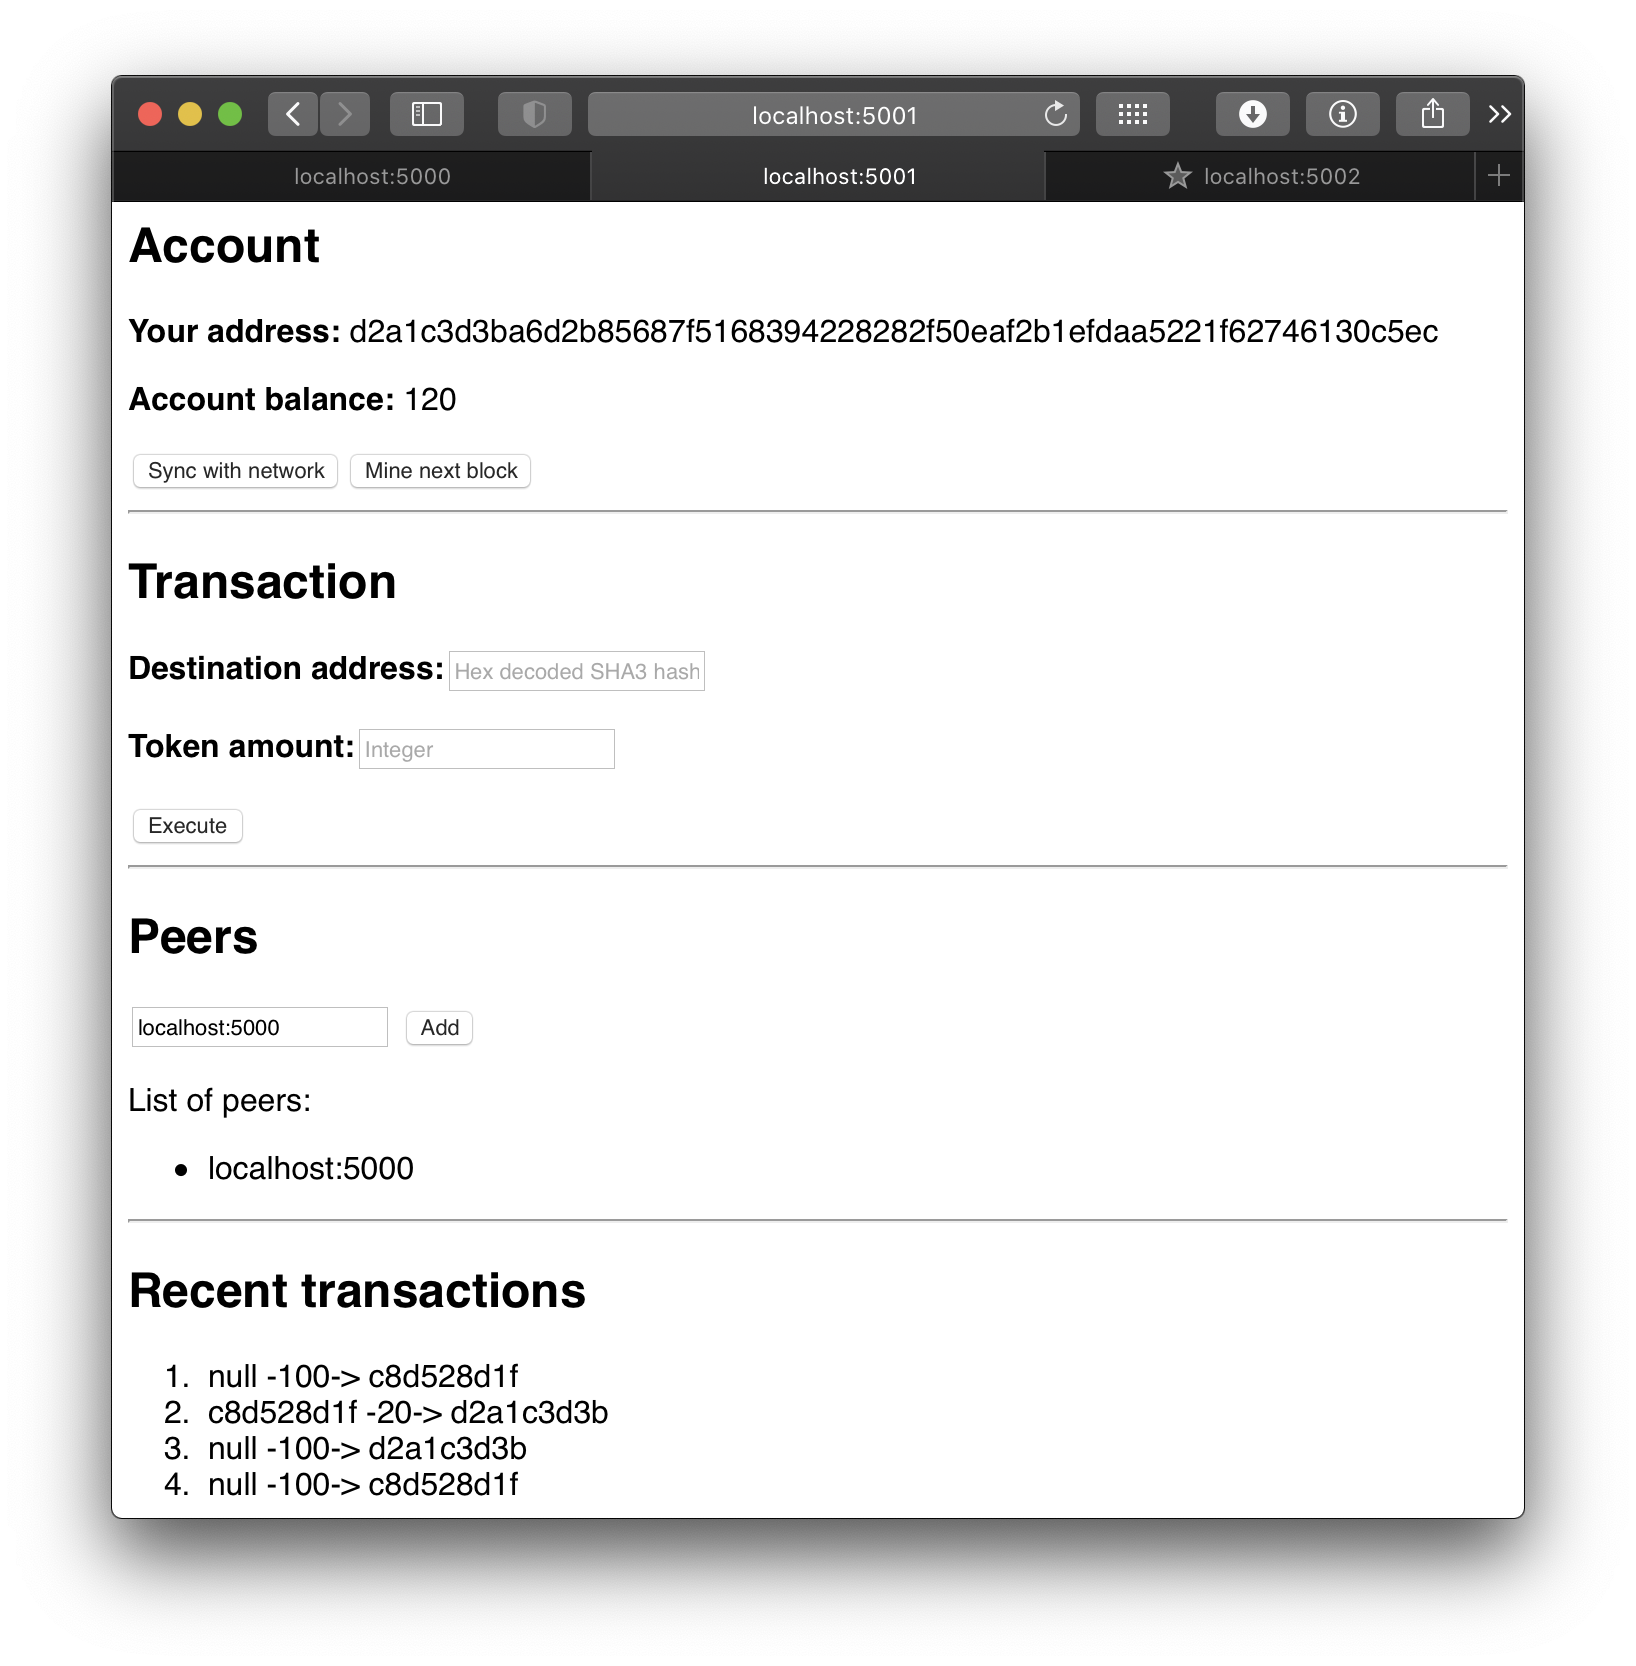
\includegraphics[width=\textwidth]{sinkronizacija.png}
    \caption{Sinkronizacija s početnim čvorom kako bismo vidjeli primljeni iznos}
    \label{fig:sinkronizacija}
\end{figure}

Možemo još nekoliku puta na jedno od klijenata pritisnuti \keys{Sync} kako bismo napravili dulji lanac na njemu. Zatim u programu trećeg klijenta dodamo 1. i 2. susjednog čvora. On će pri sinkronizaciji zatražiti informacije o lancima oba klijenta i prihvatiti najdulji važeći lanac kao autoritativan. Ukoliko bi čvor pokušao podmetnuti lanac sa nevaljanim digitalnim potpisima ili sažetcima stranica, verifikacija bi pala i ignorirali bismo lanac.

\begin{figure}[H]
    \centering
    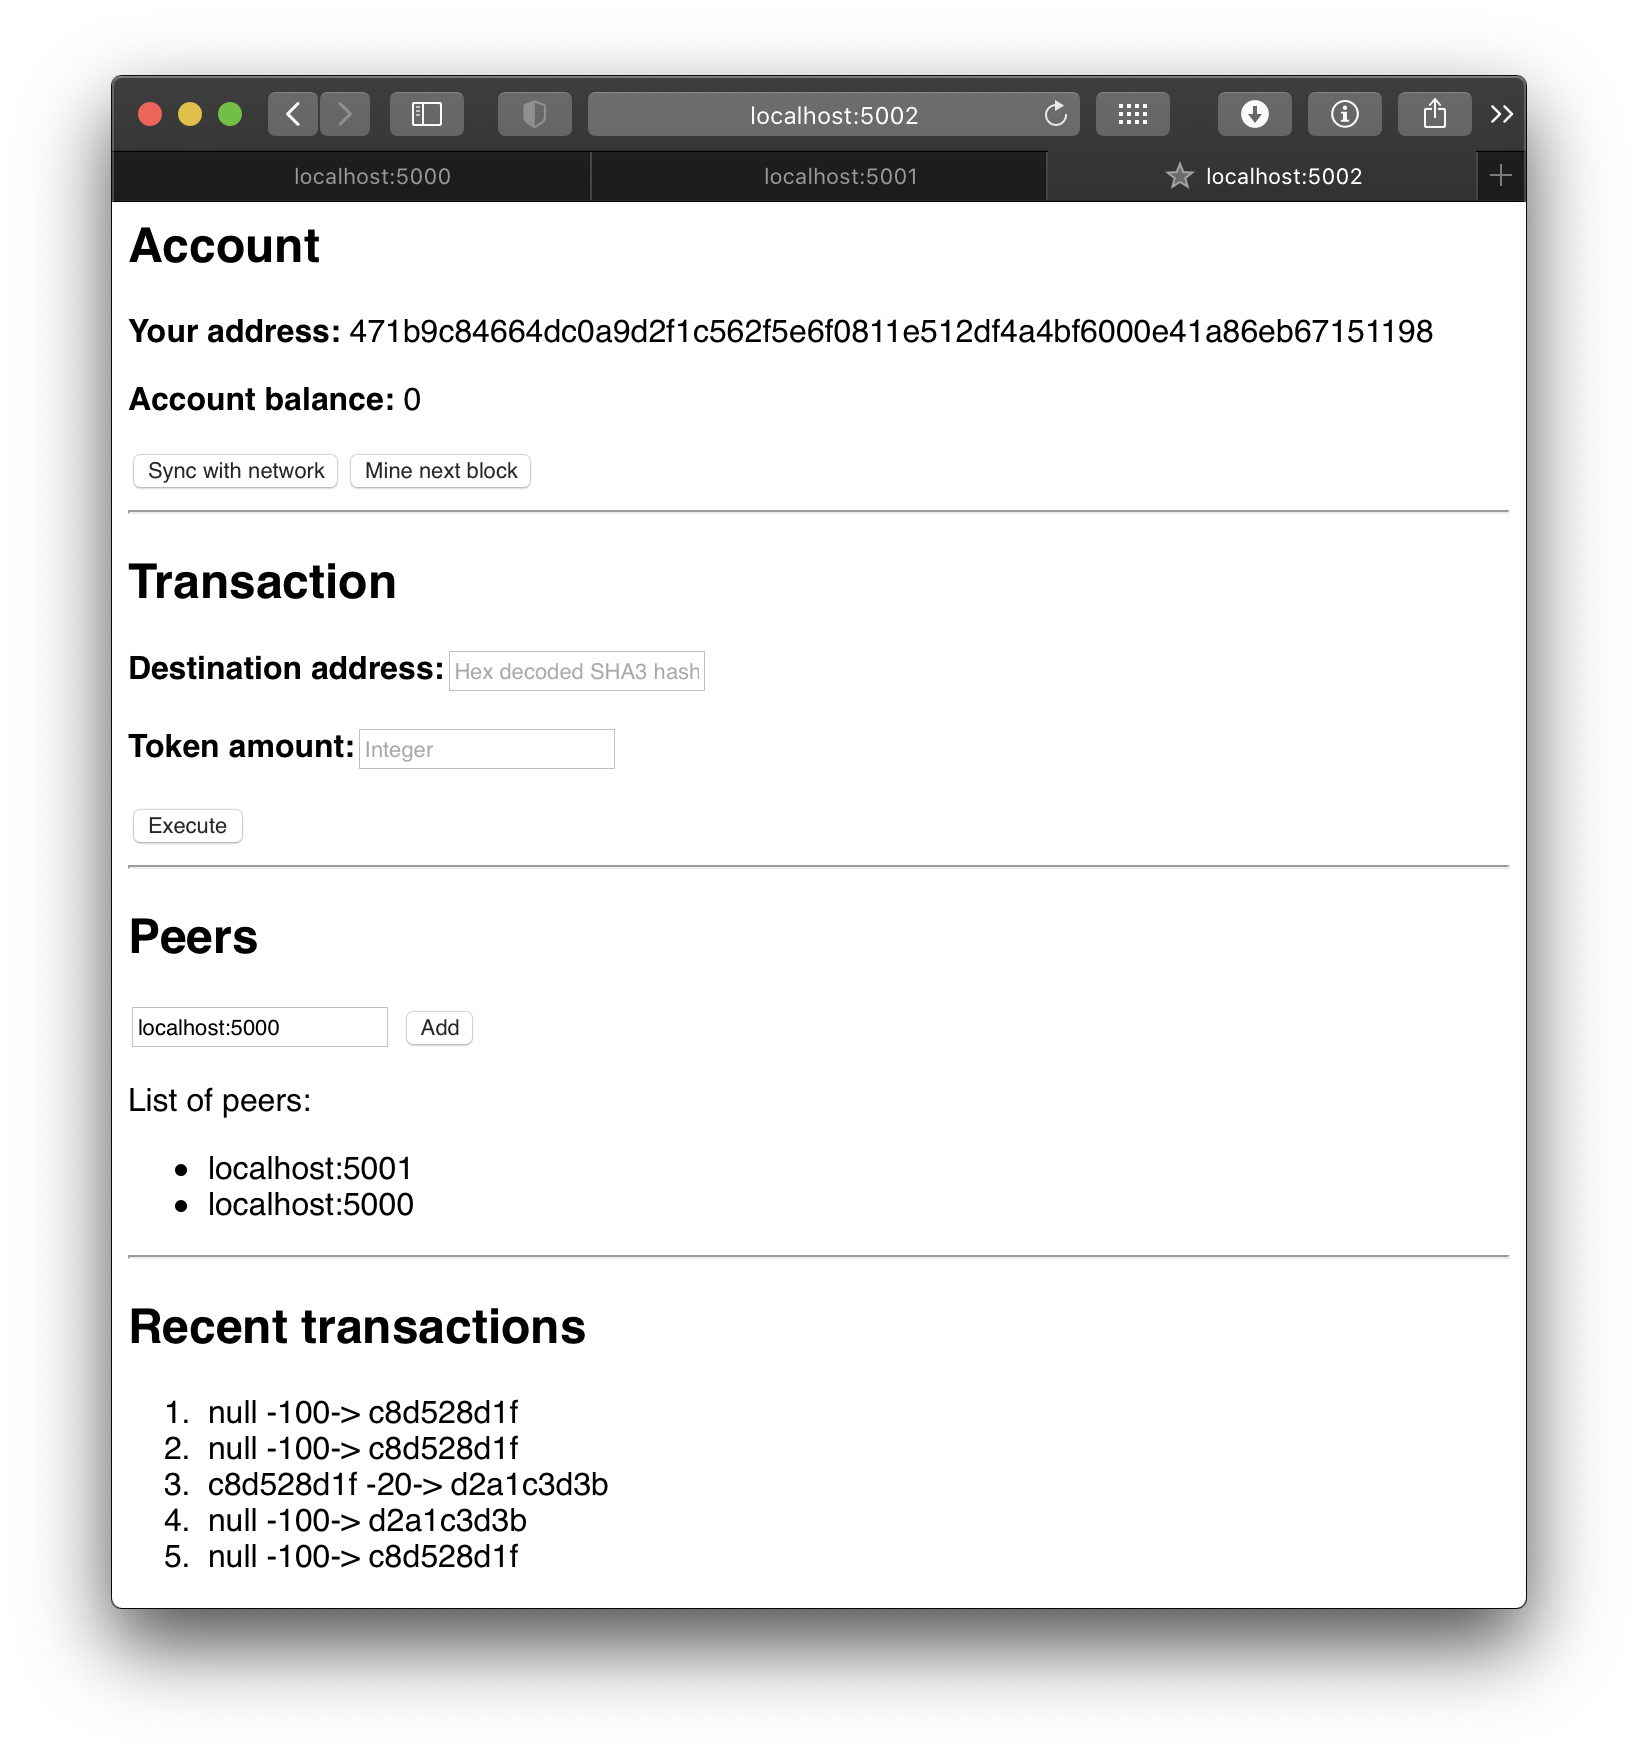
\includegraphics[width=\textwidth]{autoritativni_najdulji_lanac.png}
    \caption{Odabir autoritativnog lanca na trećem čvoru}
    \label{fig:autoritativni}
\end{figure}

% =========================
\chapter{Zaključak}
Budućnost elektroničkog novca je otvoren problem koji nema ispravnog i neispravnog rješenja. Imamo brojne obećavajuće radne okvire zasnivane na lancima stranica, prototipove i sustave u pogonu koji demonstriraju neke od potencijalnih smjerova u kojima ljudska ekonomija može otići. Lanac stranica nam nudi svježi pogled na problem upravljanja novcem, a u kombinaciji s pametnim ugovorima i linearnim skaliranjem dokaza uloga, ima potencijal da preuzme ulogu univerzalnog sustava novca. Živimo u vremenu kad je ova tehnologija u svom začetku. Prva ideja lanca stranica pojavila se 1991. kako bi 2009. prvi put ušla u praktičnu primjenu sa Bitcoin mrežom, a 2015. se javili ozbiljni konkurenti poput platforme Ethereum koji proširuje i revolucionarizira tu osnovnu ideju lanca stranica.

(TODO: dopuniti)

\bibliographystyle{fer}
\bibliography{literatura}


\begin{sazetak}
	Obrađujemo temu lanca stranica, simuliramo rad jednostavne kriptovalute te postizanje suglasja između više čvorova u mreži. Objasnit ćemo pojmove središnjeg autoriteta, suglasja u sustavima bez povjerenja, digitalnog potpisivanja, potvrđivanja transakcija i pametnih ugovora u sustavima lanca stranica.

\kljucnerijeci{Lanac stranica, distribuirano suglasje, digitalni potpis, elektronički novac, pametni ugovori}
\end{sazetak}

% TODO: Navedite naslov na engleskom jeziku.
\engtitle{Blockchain and distributed consensus in electronic money systems}
\begin{abstract}
    We analyze the topic of blockchain, simulate a simple cryptocurrency between multiple nodes in a network which achieve consensus on the state of the system. We shall formally define the concepts of central authority, consensus in trustless systems, digital signatures, validating transactions and smart contracts in blockchain systems.

\keywords{Blockchain, distributed consensus, digital signature, electronic money, smart contract}
\end{abstract}

\end{document}